\renewcommand{\chaptername}{}
\chapter{Markov Chain }
\ifpdf
    \graphicspath{{MarkovChain/Chapter3Figs/PNG/}{MarkovChain/Chapter3Figs/PDF/}{MarkovChain/Chapter3Figs/}}
\else
    \graphicspath{{MarkovChain/Chapter3Figs/EPS/}{MarkovChain/Chapter3Figs/}}
\fi
\markboth{\MakeUppercase{\thechapter. Markov Chain}}{\thechapter. Markov Chain}
In this part, some properties of stochastic processes and the approach of a Markov chain to calculate the probabilities of the absorbing states  and absorbance times in such systems will be explained. Competition and natural selection in biological scenarios, which are modeled with Moran process, have the properties of such stochastic systems. This relation allows us to calculate analytically expressions for fixation probability and average time of fixation of a new mutant or group of mutants competing with the old population in two cases: random and neutral drift.  
  
 

\section{ Moran process}
This process is a stochastic model that was created by Moran to simulate selection among different types of individuals across generations in finite populations, where the organism with the largest fitness will invade the whole population depending on the initial population.   


Imagine an experiment where a population of bacteria is at its maximal carrier capacity; then the population size will be constant, and that means that when an offspring is born other individual has to die. 
This is the Moran process, where at each time step one individual of the population is chosen randomly for reproduction with a probability that depends of its fitness. In order to keep a constant population size, the new offspring replaces another individual of the population that is chosen randomly as is depicted in Figure (\ref{Fig41}). 

\begin{figure}[H]
  \begin{center}
    \leavevmode
    \ifpdf
      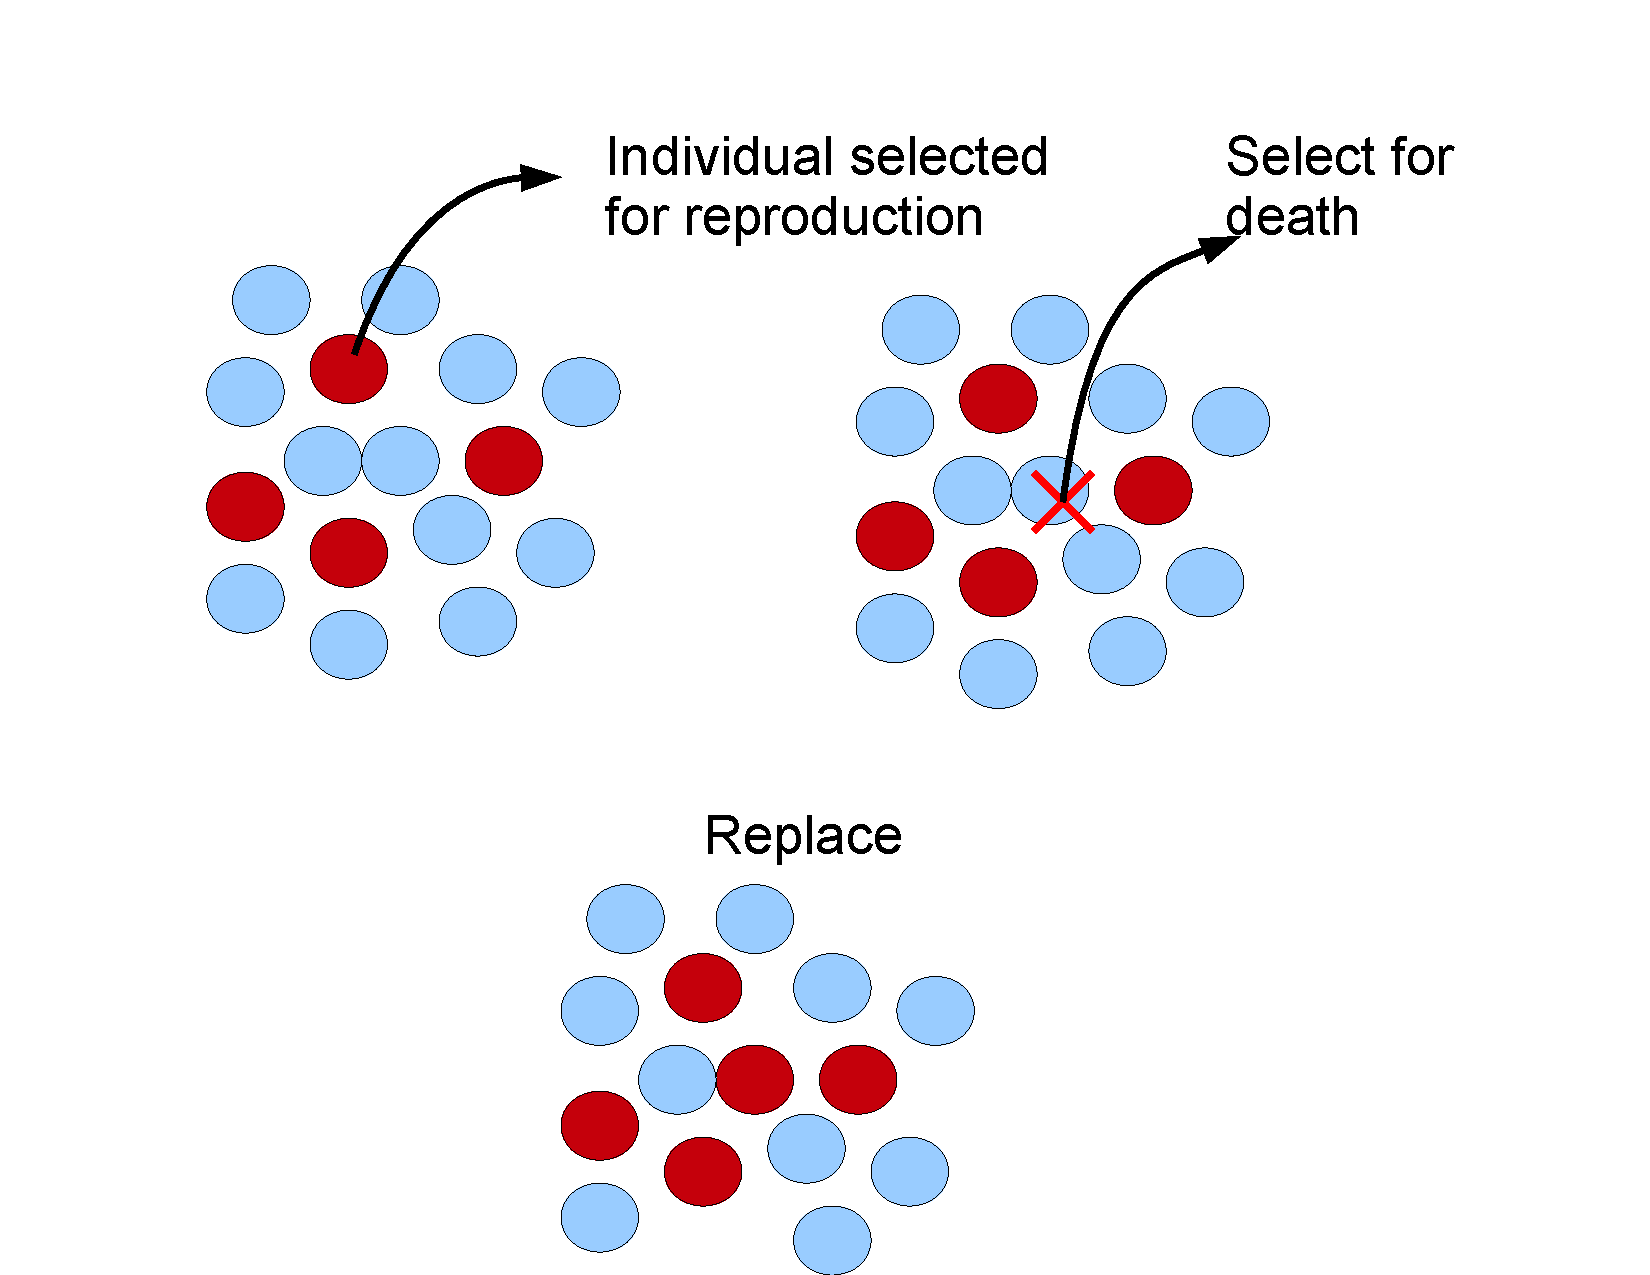
\includegraphics[width=7cm,height=5cm]{moranprocess.pdf}
    \else
      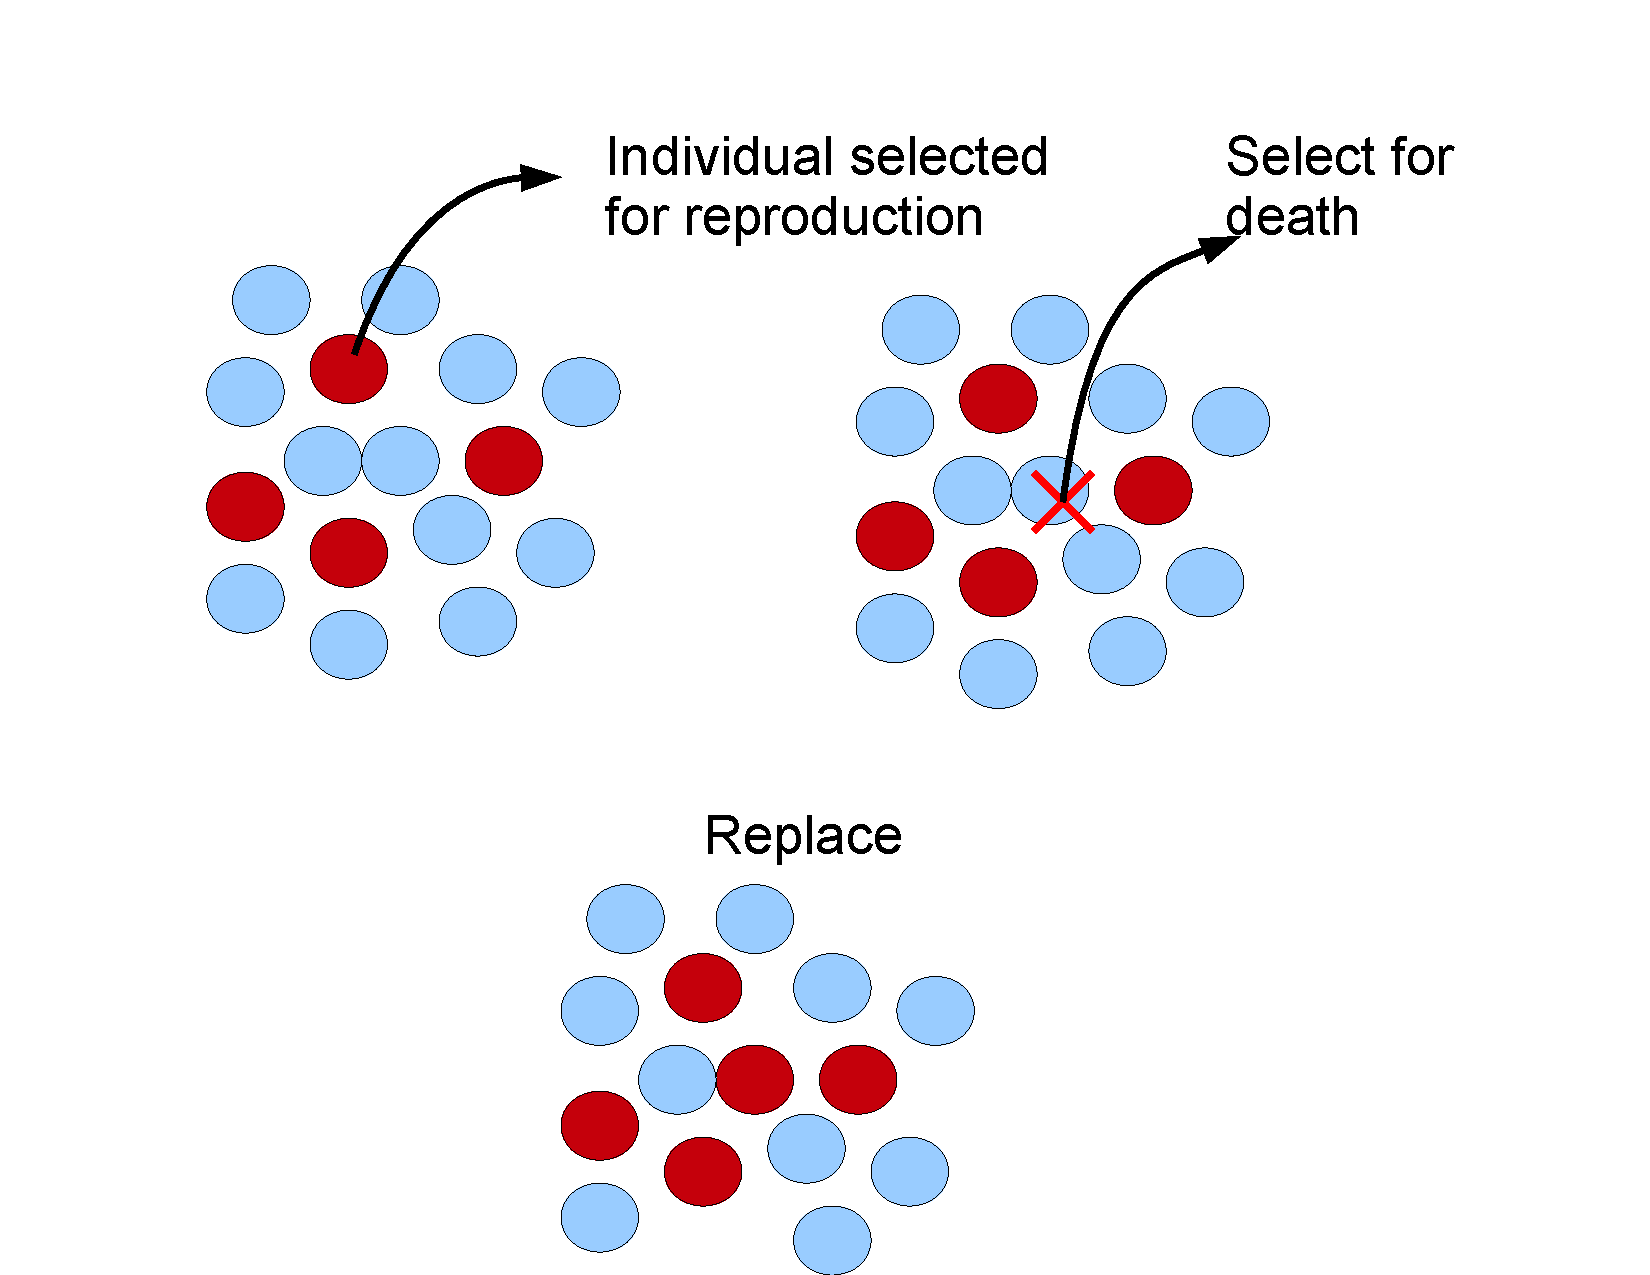
\includegraphics[width=7cm, height=5cm]{moranprocess.pdf}
    \fi
    \caption{Example of birth and death in Moran process, where it is seen that the size population is constant.}
    \label{Fig41}
  \end{center}
  \end{figure}

Because a Moran process is a birth and death process, it is a Markov chain which has two absorbing states in the case of two types competing.

What is a Markov chain? A Markov chain is a random process with a set of discrete and finite states. In this process, the transitions from one state to another occurs in discrete time steps, where the transition to the next state depends only on the present state and not on the preceding sequence of states, which is the Markov property.

The next Figure (\ref{Fig42})  is a graph that represents a Markov chain, 
\begin{figure}[H]
 \begin{center}
    \leavevmode
    \ifpdf
      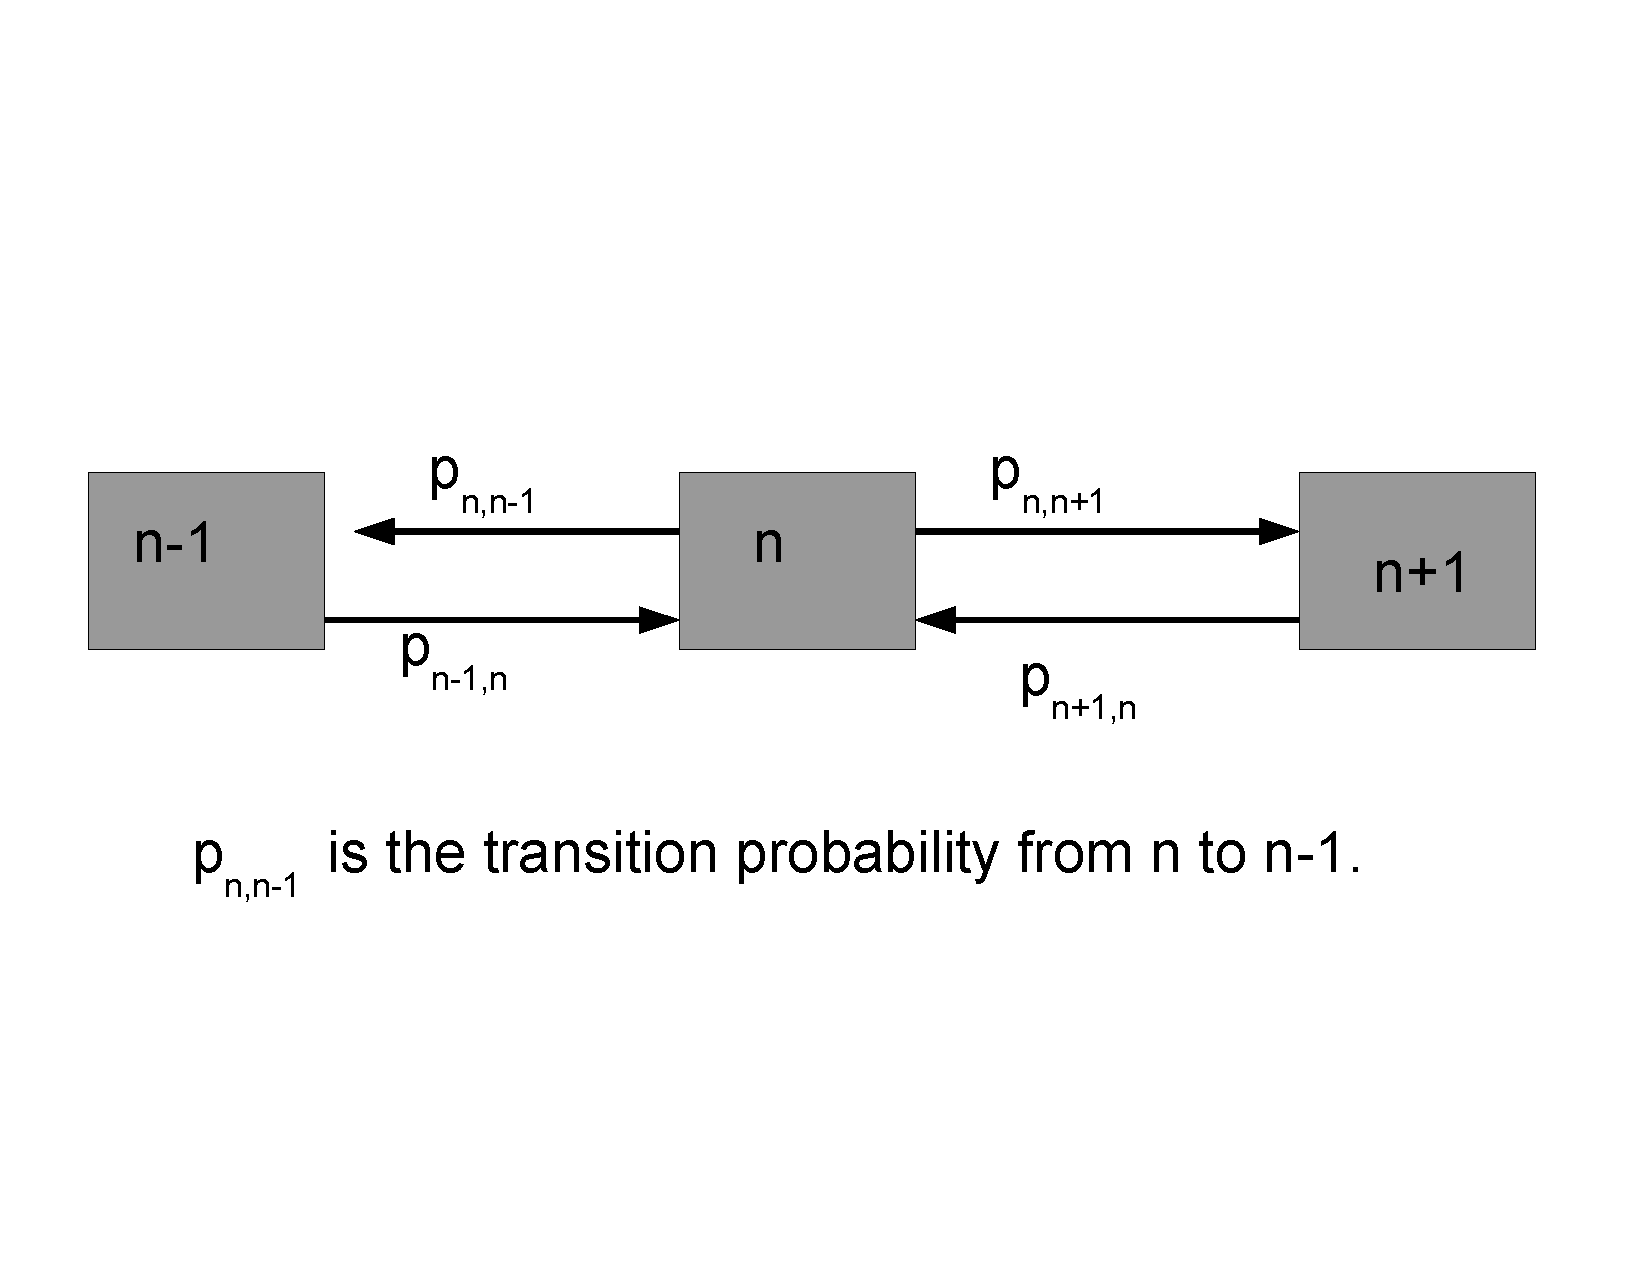
\includegraphics[width=7cm,height=5cm]{markovchain.pdf}
    \else
     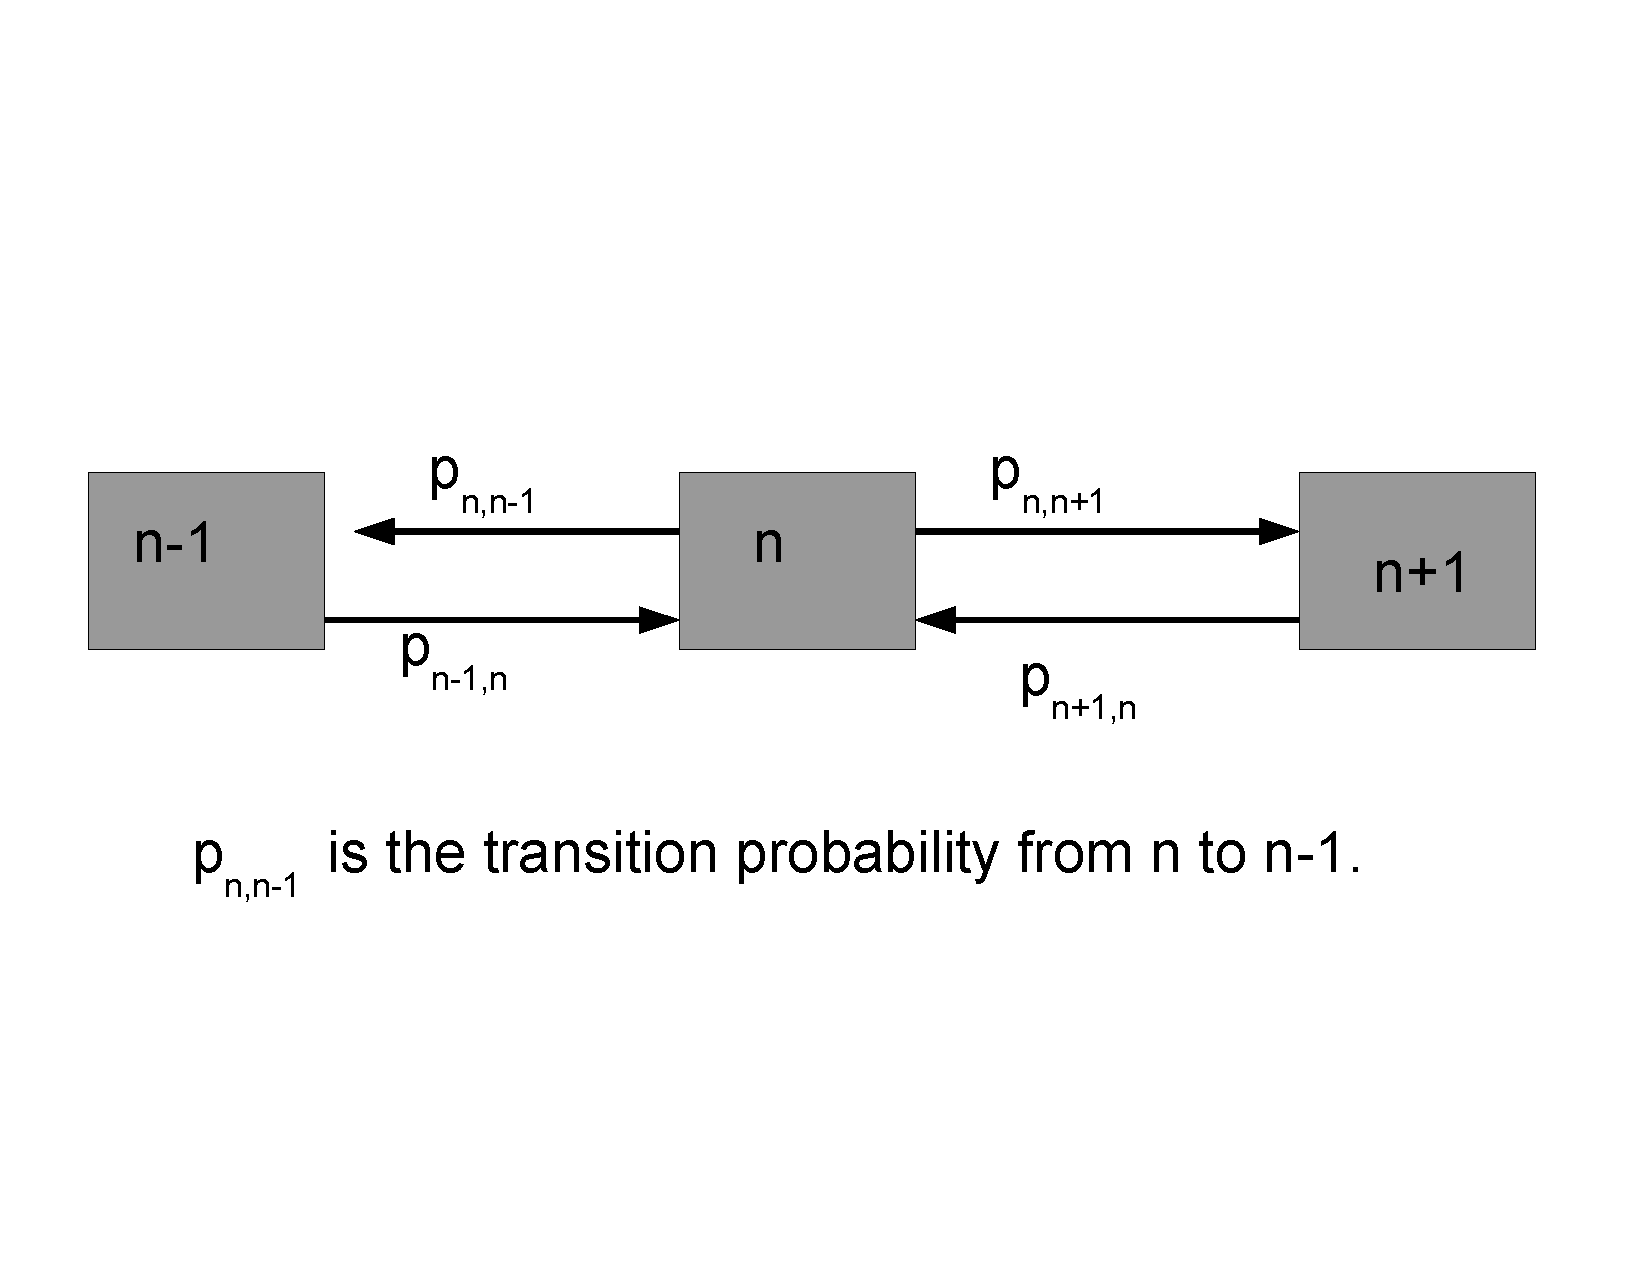
\includegraphics[width=7cm, height=5cm]{markovchain.pdf}
    \fi
    \caption{Graph of transitions in a Markov process.}
    
    \label{Fig42}
  \end{center}
  \end{figure}

where $n$, $n-1$ and $n+1$ are states of the system and the arrows represent the transition between neighbor states. The master equation for the probability flux of state $n$ is
\begin{equation}\label{4.1}
\frac{dP_{n}}{dt}=-(p_{n,n-1}+p_{n,n+1})P_{n}+p_{n-1,n}P_{n-1}+p_{n+1,n}P_{n+1}.
\end{equation} 
Now let us see the Markov graph representation for a simple Moran process in a population of size $N$ and two different organisms of type $A$ and $B$ Figure (\ref{Fig43}), where $n$ is the number of individuals of type $A$(red balls) and the system have a  population size $N=14$, the fitnesses for the two types are $f_{A}$ and $f_{B}$.
\begin{figure}[H]
 \begin{center}
    \leavevmode
    \ifpdf
      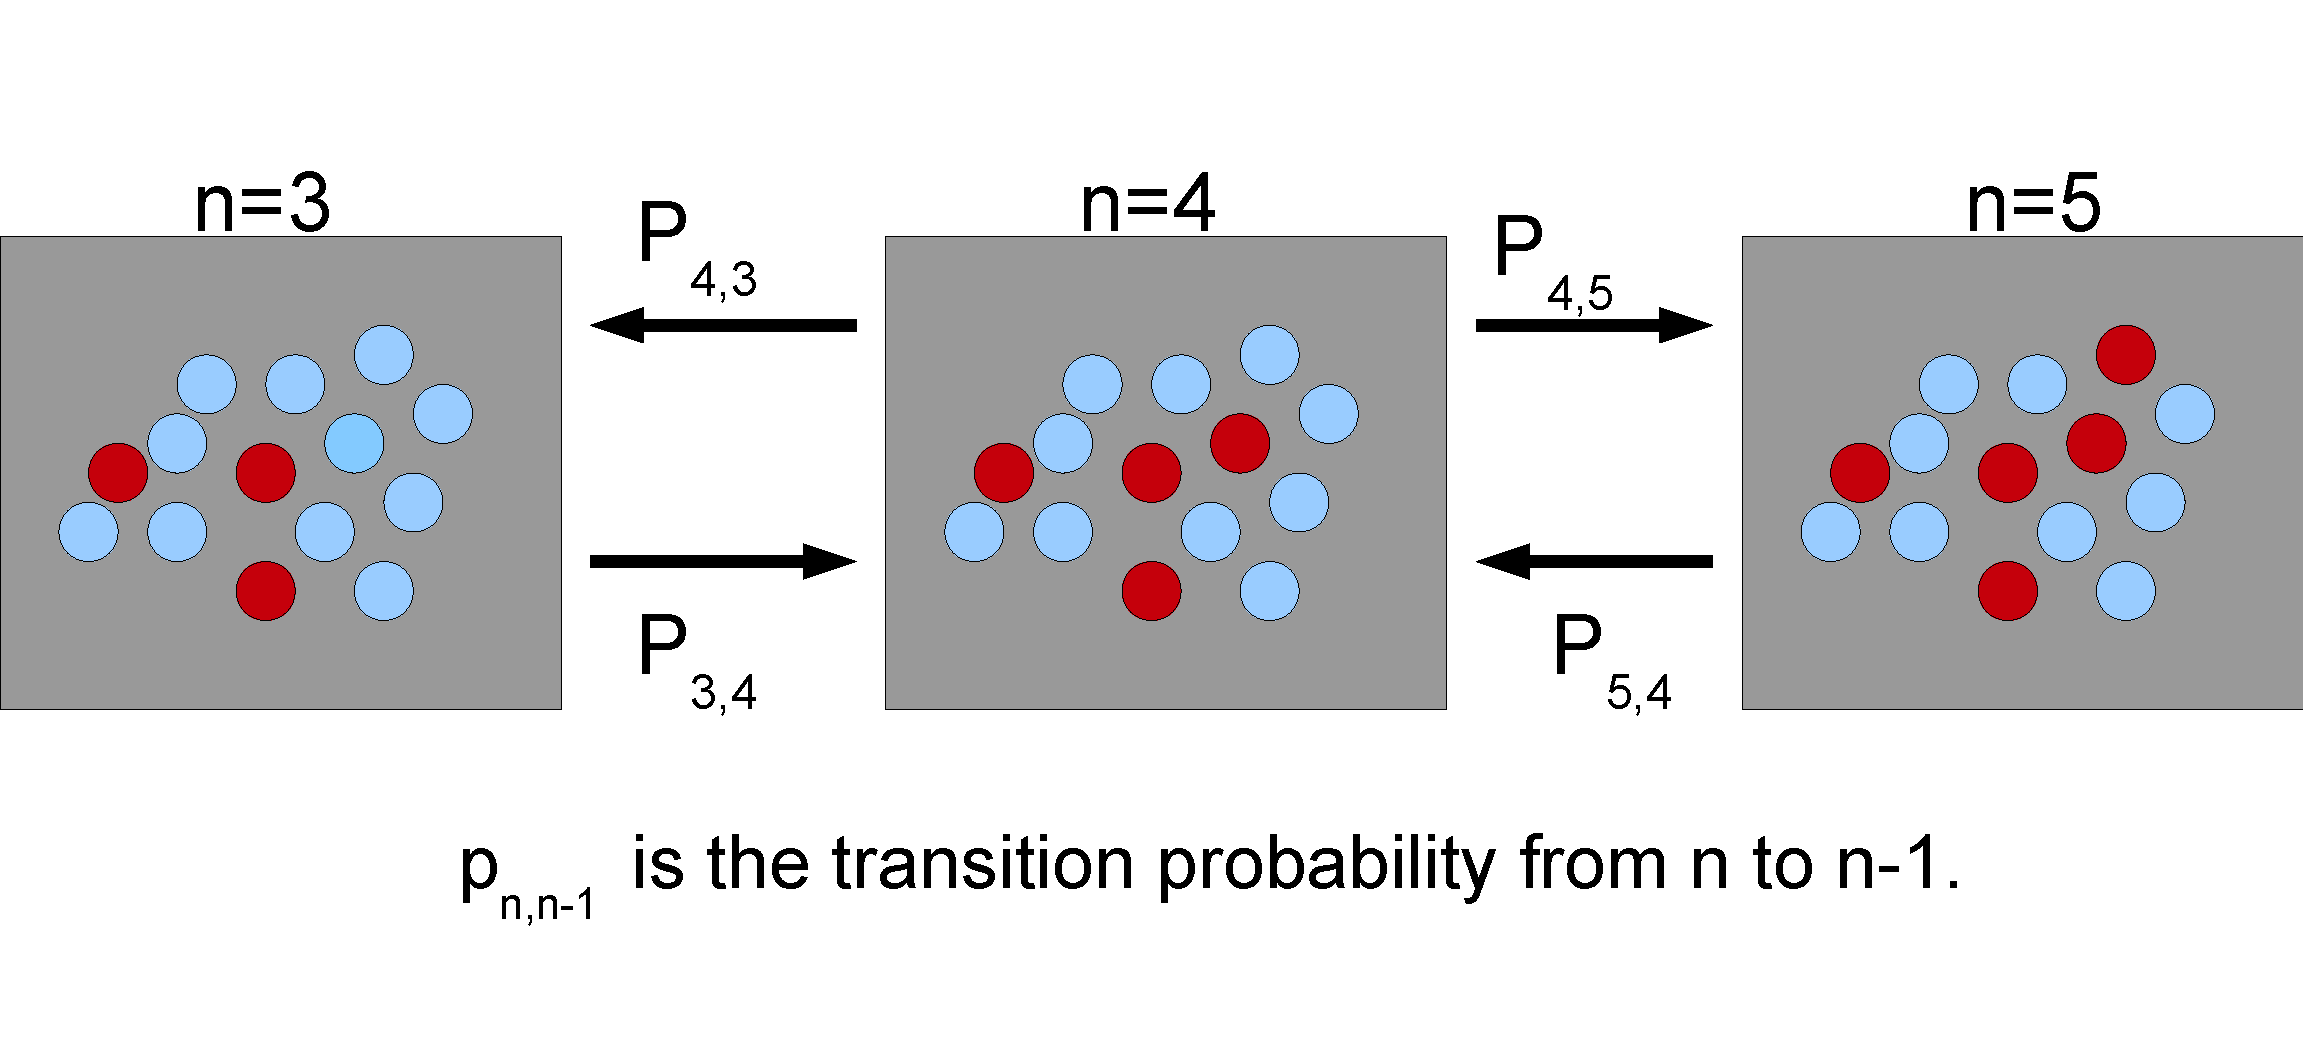
\includegraphics[width=9cm,height=7cm]{markovchainMoran.pdf}
    \else
     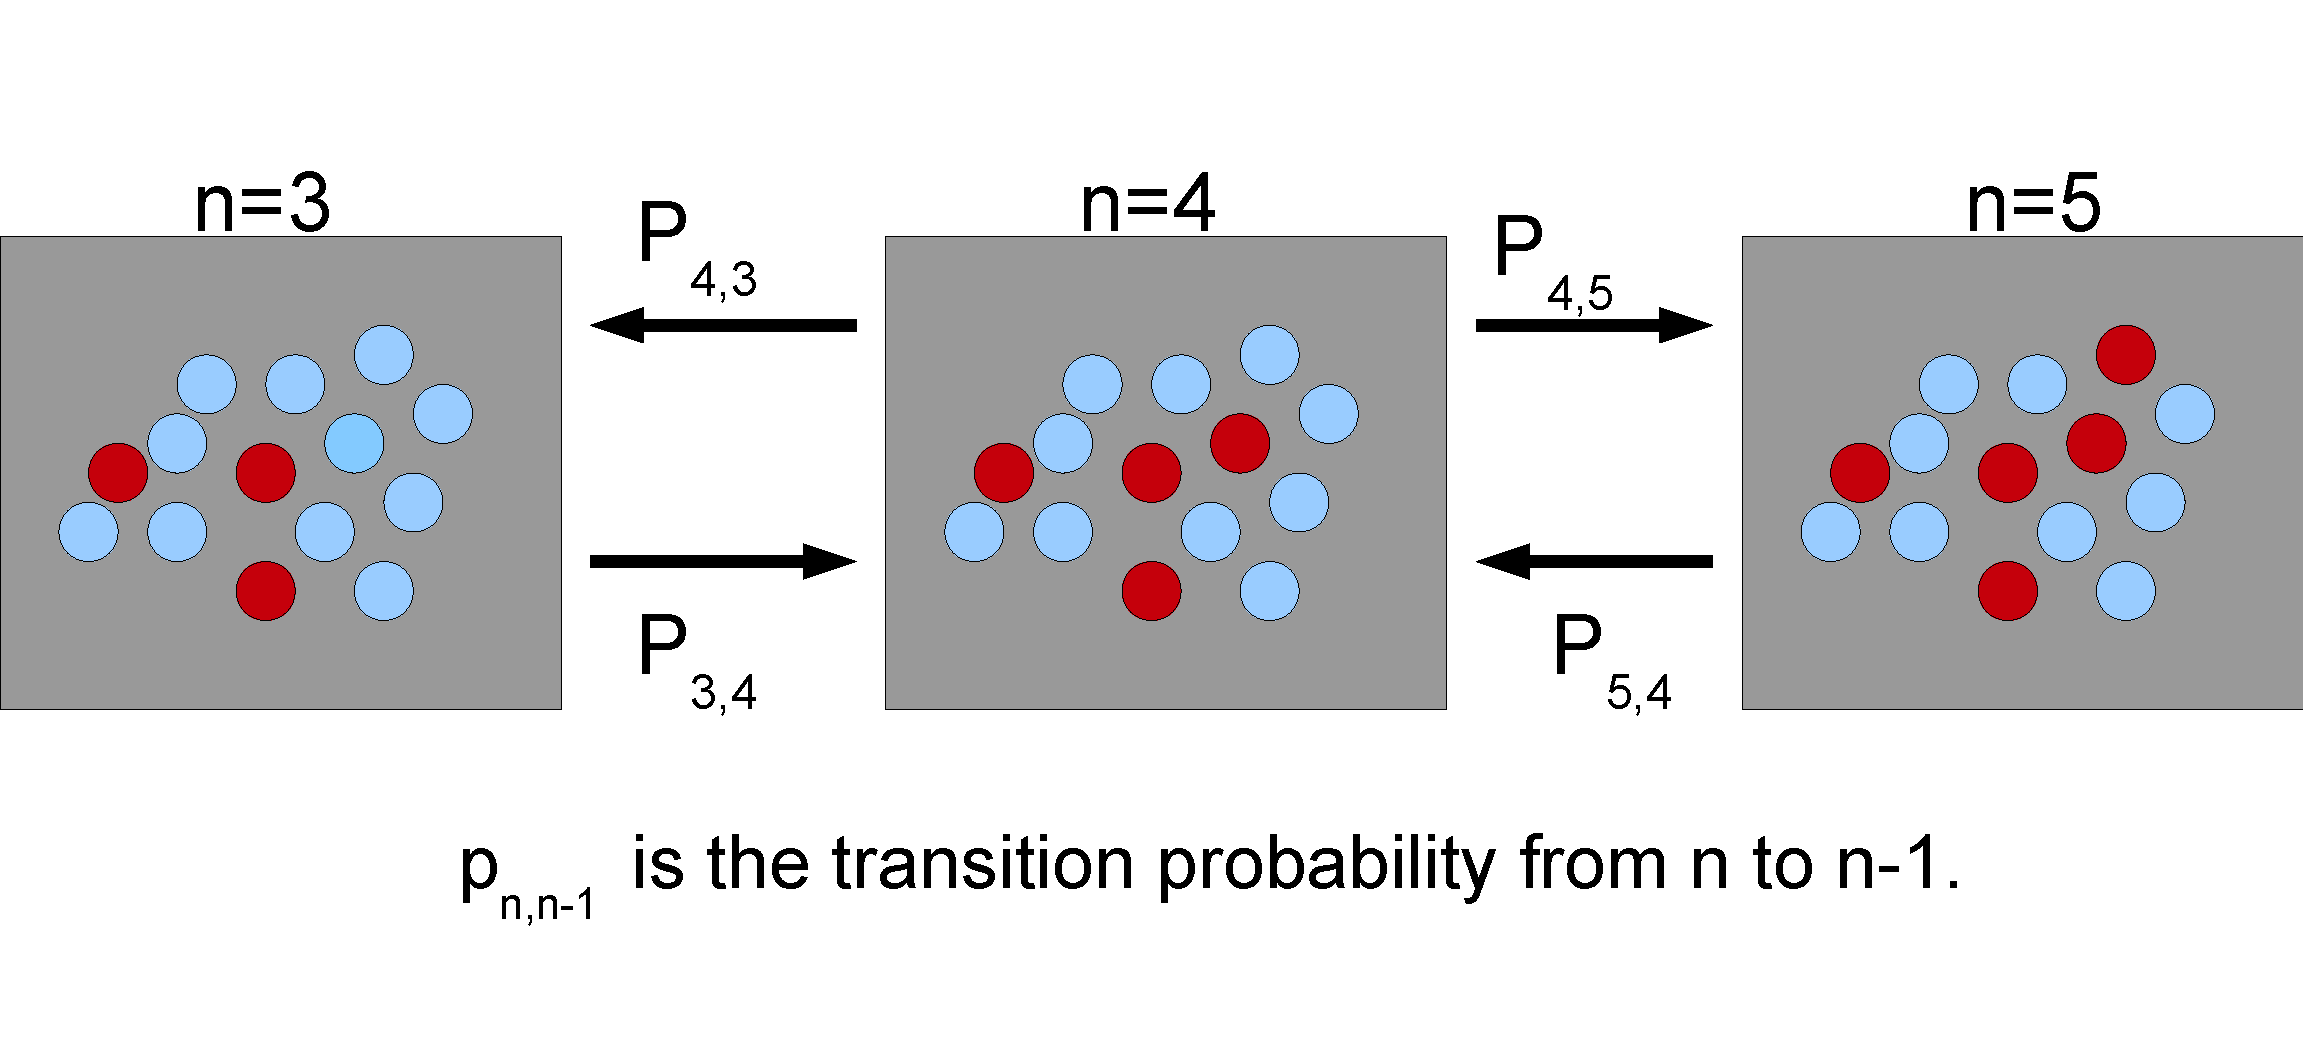
\includegraphics[width=9cm, height=7cm]{markovchainMoran.pdf}
    \fi
    \caption{Graph of transitions in a simple Moran process.}
    \label{Fig43}
  \end{center}
  \end{figure}

The probabilities of being selected for reproduction are $p_{A}$ and $p_{B}$, with the condition $p_{A}+p_{B}=1$, and each one is proportional to the type`s fitness, usually a linear function\cite{Shoresh2011}.
\begin{equation}
p_{A}=\frac{f_{A}n}{f_{A}n+f_{B}(N-n)} \;\; , \;\; p_{B}=\frac{f_{B}(N-n)}{f_{A}n+f_{B}(N-n)}.
\end{equation}  
The individual selected to die is chosen randomly, so the probabilities of  death for $A$ and $B$ are
\begin{equation}
\frac{n}{N}\;\;\; , \;\;\; \frac{N-n}{N}
\end{equation}
respectively. Therefore the probabilities of transition are
\begin{equation}
p_{n,n+1}=\frac{f_{A}n}{f_{A}n+f_{B}(N-n)} \frac{N-n}{N} \;\;\; , \;\;\; p_{n,n-1}=\frac{f_{B}(N-n)}{f_{A}n+f_{B}(N-n)}\frac{n}{N}
\end{equation}
and 
\begin{equation}
p_{n,n}=1-p_{n,n-1}-p_{n,n+1}
\end{equation}
In the next simulation Figure (\ref{Fig44}) we show the population of $A$ individuals as a function of time for a stochastic simulation of the Moran process. This stochastic simulation is a Monte Carlo step algorithm written in C++.
\begin{figure}[H]
 \begin{center}
    \leavevmode
    \ifpdf
      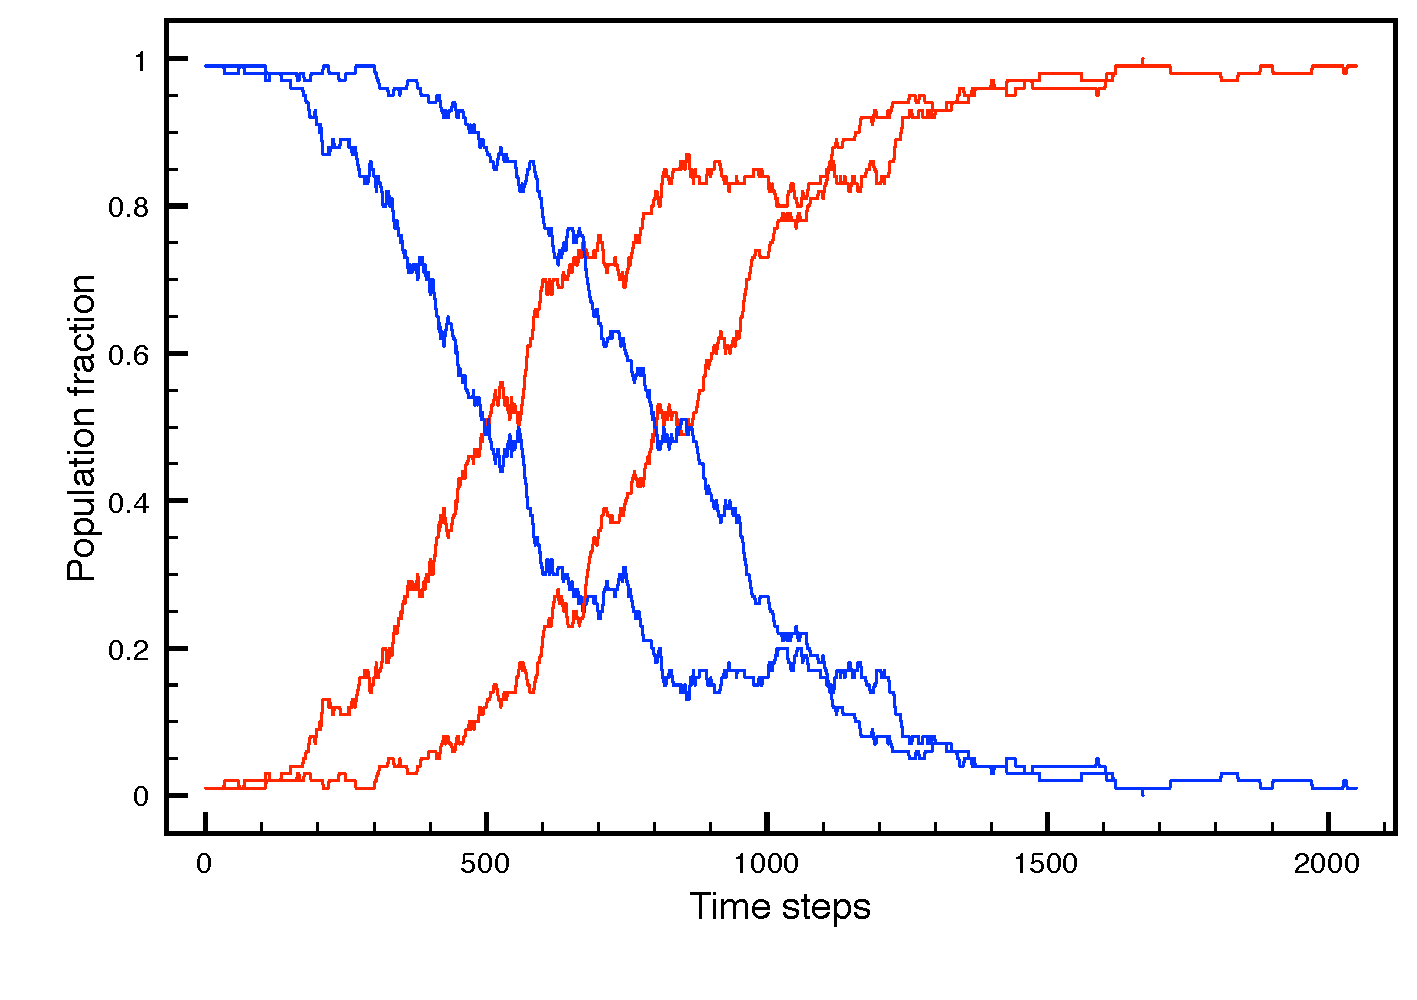
\includegraphics[width=10cm,height=7cm]{moransimulation.pdf}
    \else
     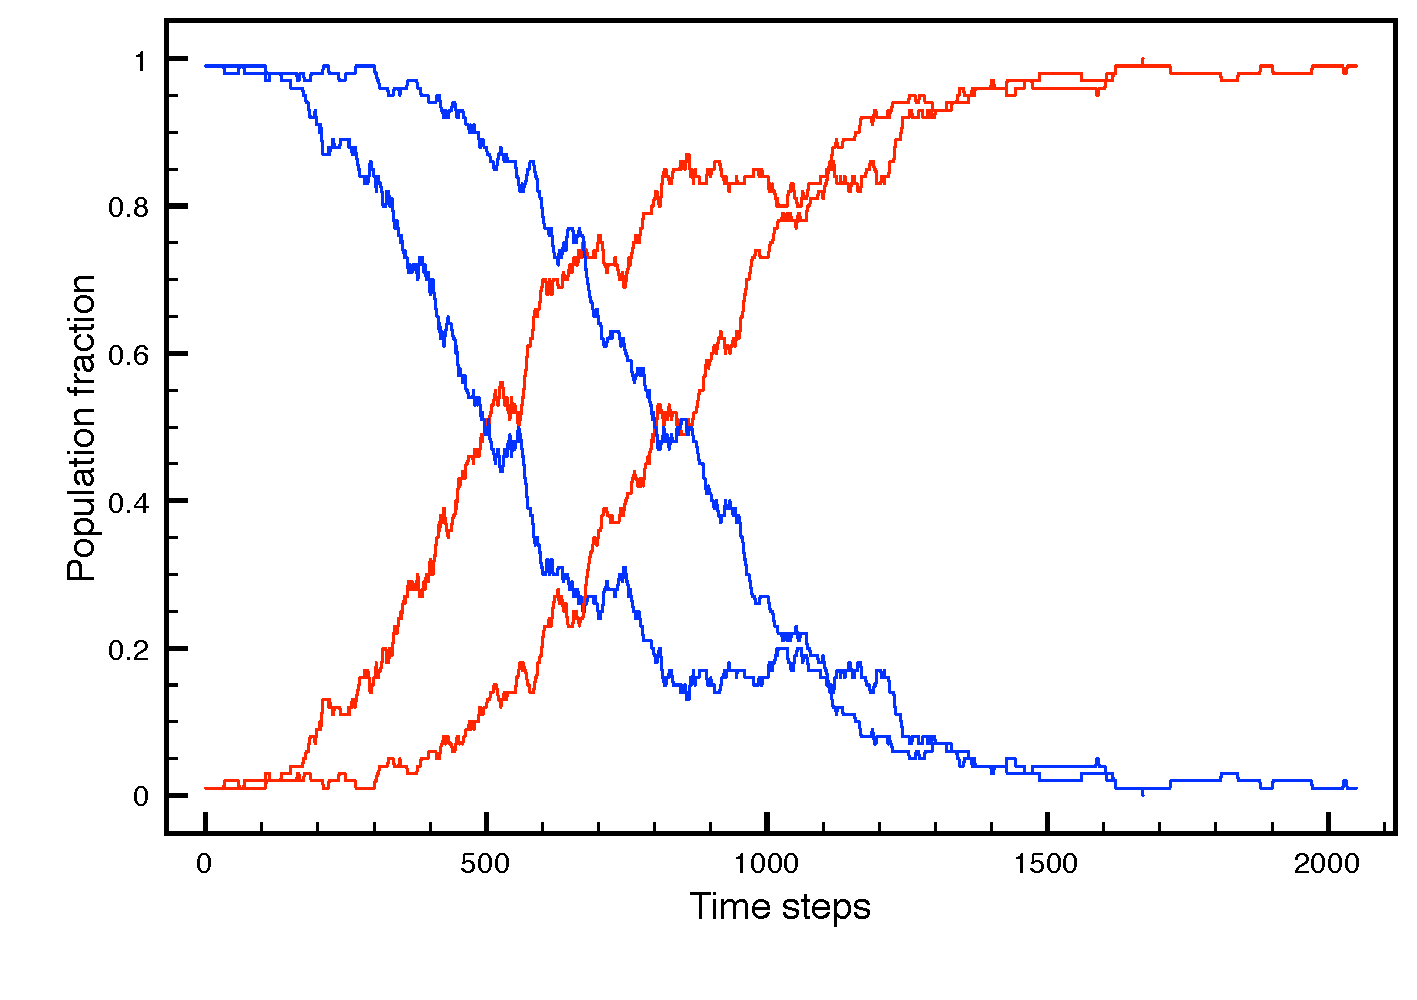
\includegraphics[width=10cm, height=7cm]{moransimulation.pdf}
    \fi
    \caption{\footnotesize Stochastic simulation of the Moran process for two executions of the program(Randomdrift.cpp). Blue line represents the population of $B$ individuals and red $A$ individuals. The fitnesses are $f_{A}=2$, $f_{B}=1$ and $N=100$ with an initial population of $A$ individuals $i=1$.}
    \label{Fig44}
  \end{center}
  \end{figure}
Now imagine that you have an experiment where you have $m>>1$ boxes with medium for growth bacterias, and in each of them you set the same initial conditions of population for two different types of bacterias. Then you let them compete until they have reached dominance in each box. 

\begin{figure}[H]
 \begin{center}
    \leavevmode
    \ifpdf
      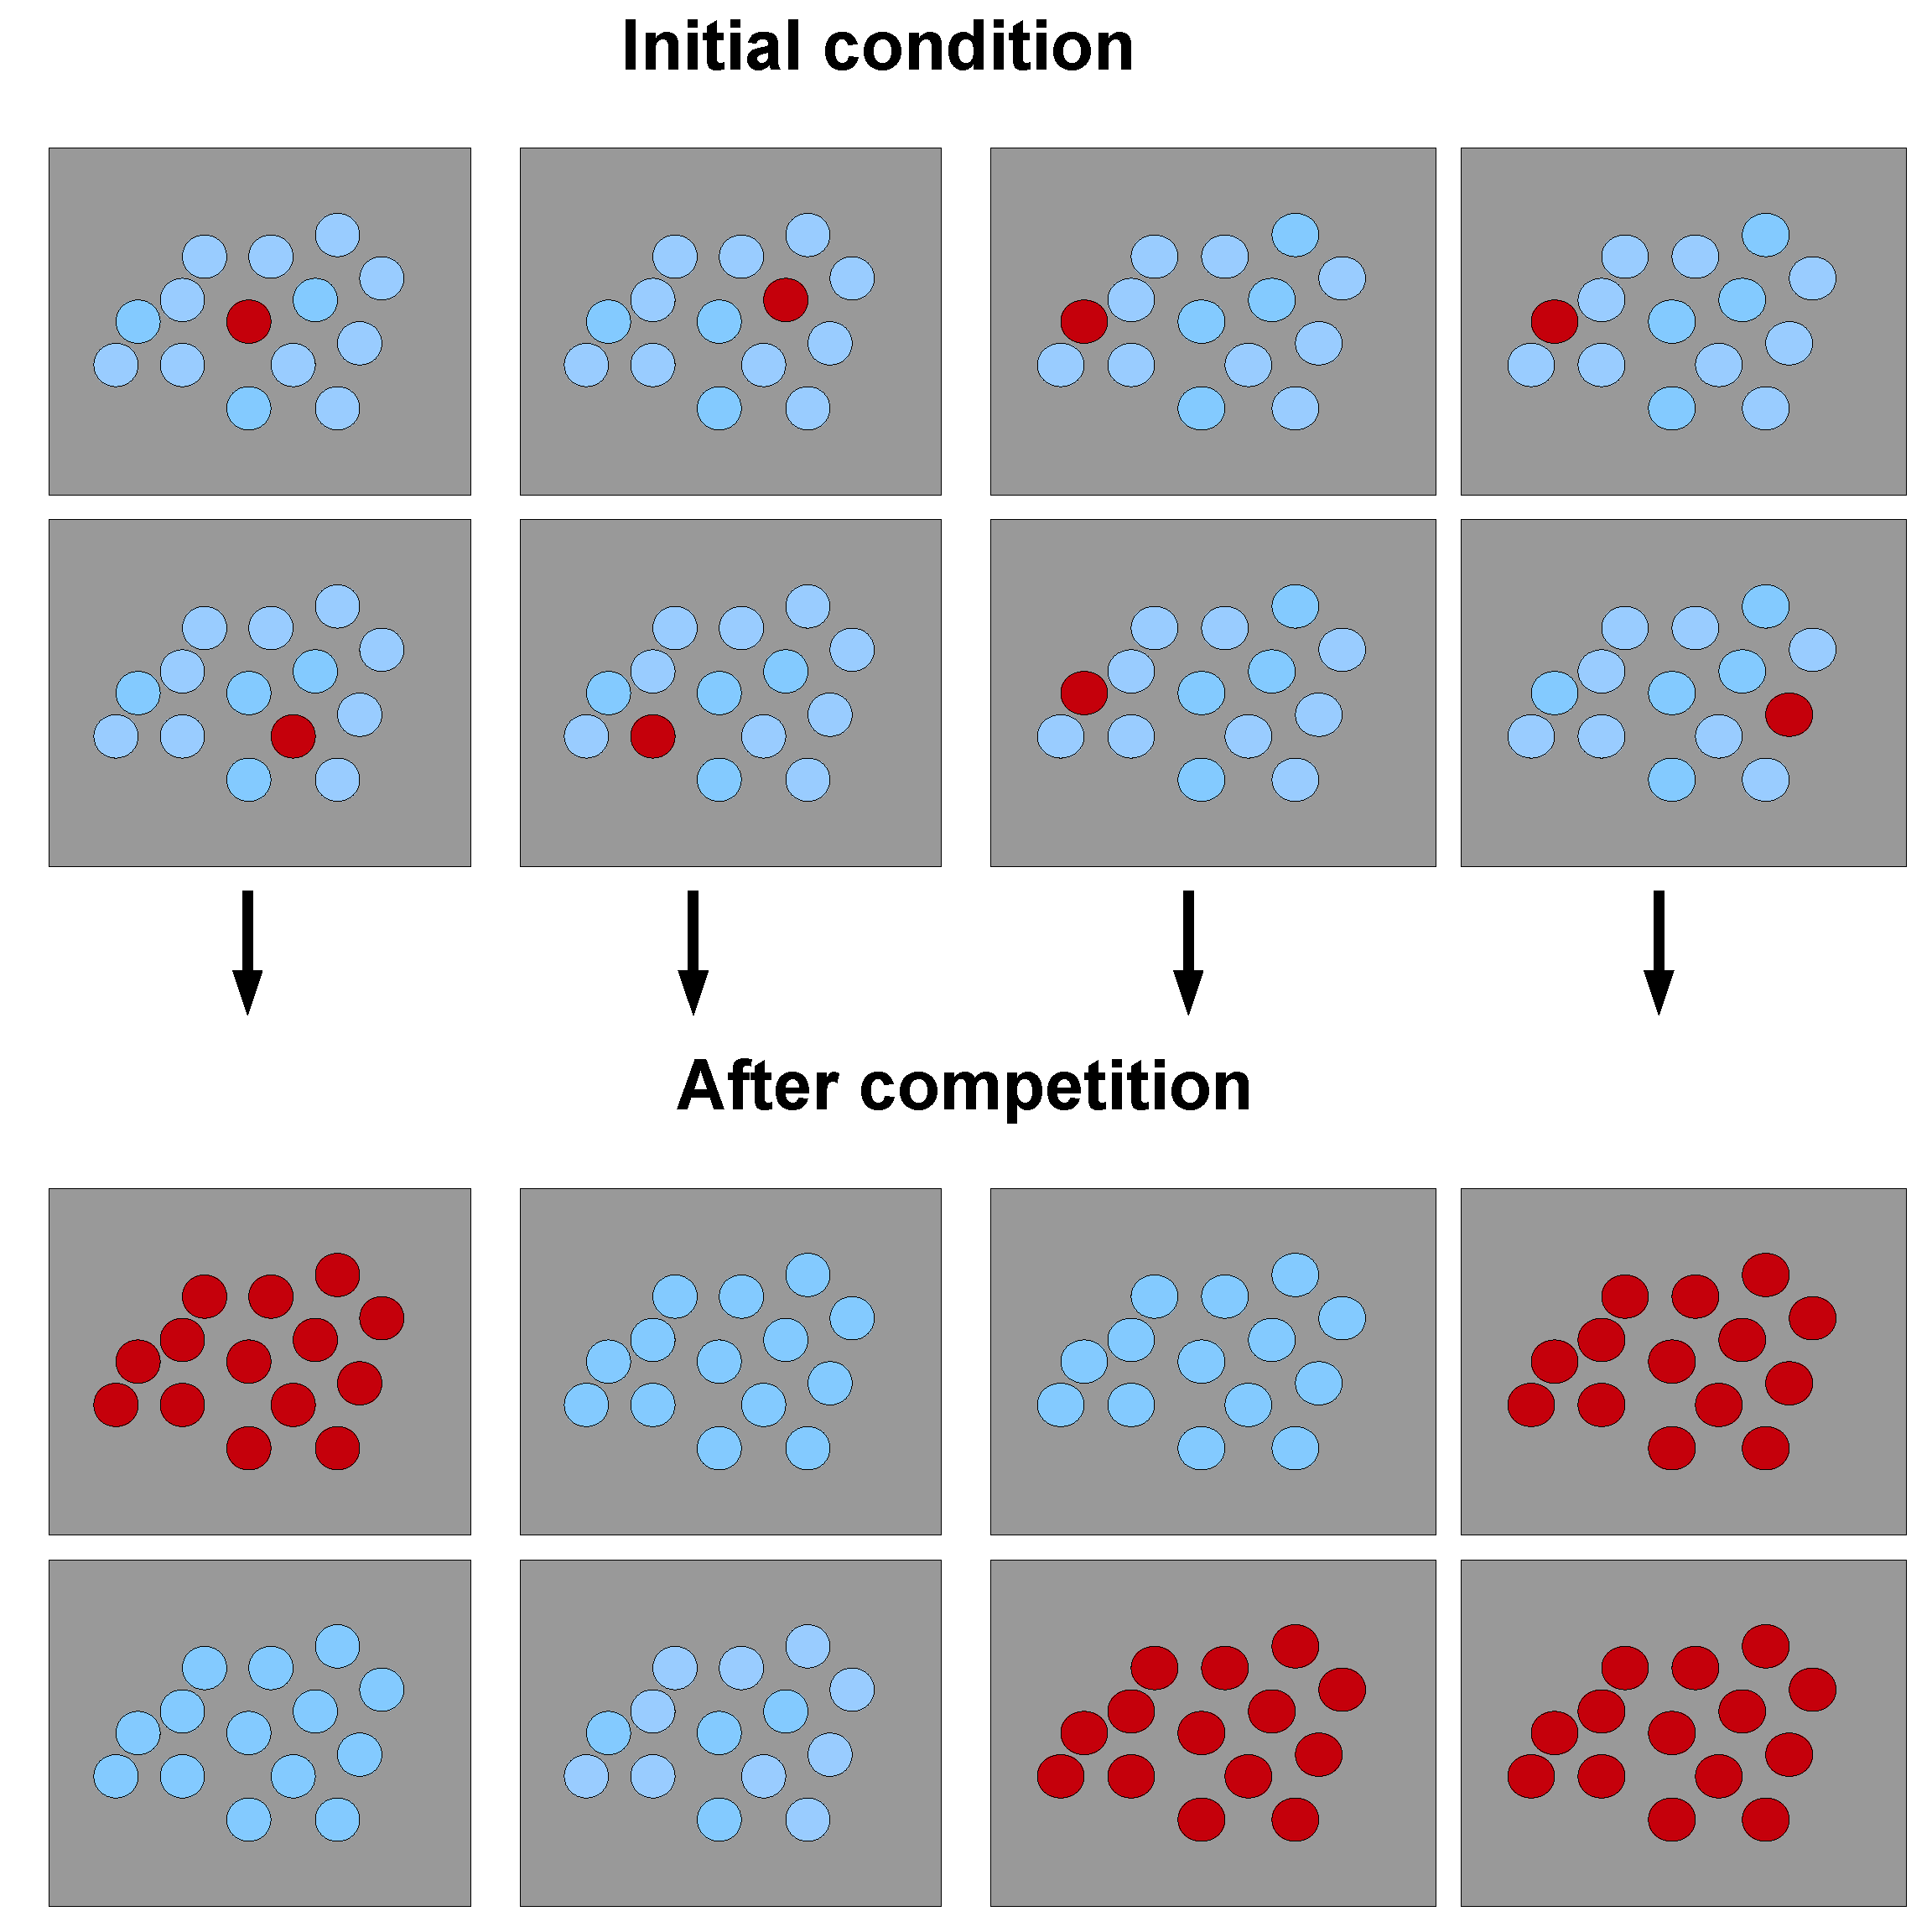
\includegraphics[width=10cm,height=7cm]{array.pdf}
    \else
     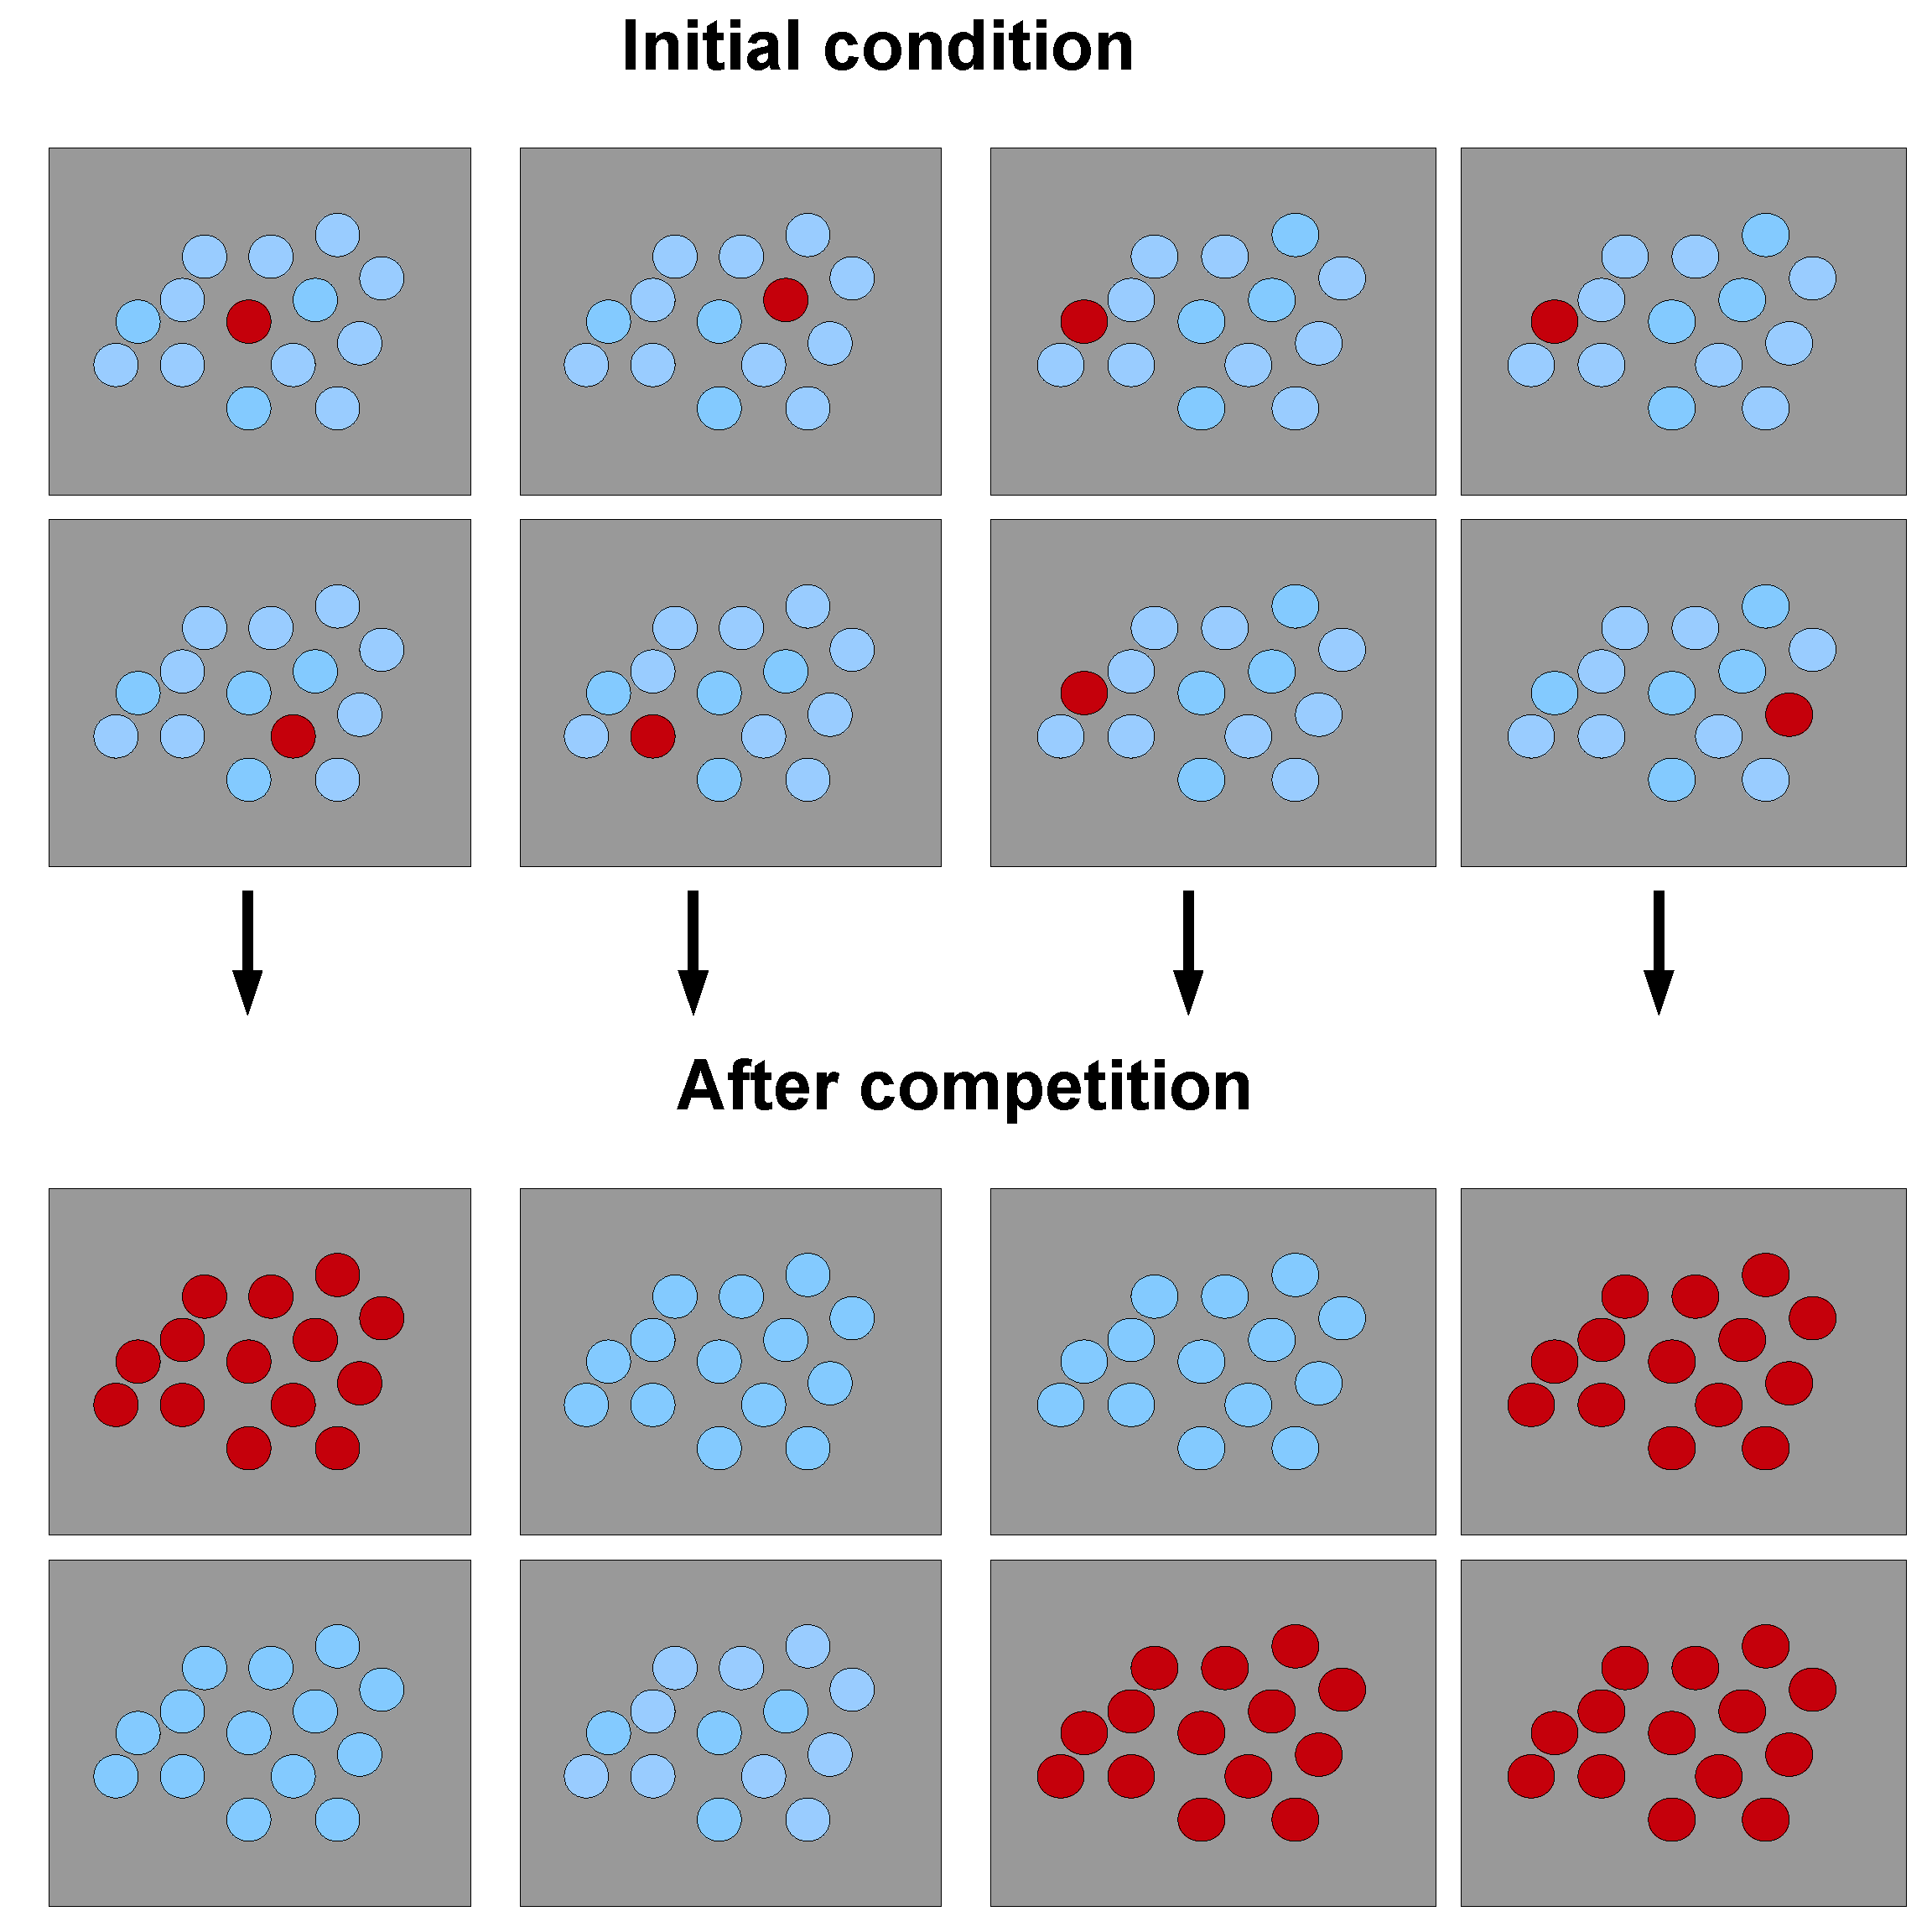
\includegraphics[width=10cm, height=7cm]{array.pdf}
    \fi
    \caption{\footnotesize Representation of several boxes with the same initial conditions that have different final states because of the stochasticity. The fraction of boxes where $A$ wins is called fixation probability.}  
    \label{Fig45}
  \end{center}
  \end{figure}


This is equivalent to running several times a simulation with the same initial conditions. Because of the stochasticity there is a fraction of boxes where each type dominate, but not in all, and this fraction is called the fixation probability for that respective type. It can be calculated analytically by solving the follow recurrence   equation for $\rho_{i}$ the fixation probability.
\begin{equation}
\rho_{i}=p_{i,i+1}\rho_{i+1}+p_{i,i-1}\rho_{i-1}+p_{i,i}\rho_{i}.
\end{equation} 
where $i$ is the initial population of individuals of type $A$.
\section{Neutral Drift}
In neutral drift two different types of organisms have equal fitnesses, so the dominance of one of them will depend only on the frequency of each type.  

The analytical procedure to find the probability of dominance is as follows: With a population of size $n$ and $i$ individuals of type $1$, the probabilities of choosing are: $i/n$ for type $1$ and $(n-i)/n$ for type $0$. Then the probability  that the population changes from $i$  to $i+1$ is 
\begin{equation}
p_{i,i+1}=\frac{i(n-i)}{n^2},
\end{equation}   
and from $i$ to $i+1$ is
\begin{equation}
p_{i,i-1}=\frac{(n-i)i}{n^2}.
\end{equation}
 The probability $\rho_i$ of fixation or dominance for the initial condition of $i$ individuals of type $1$ is $\rho_i=0$ if $i=0$ and $\rho_i=1$ if $i=n$; this is because  when an individual is chosen to die it is replaced by one of its same type. The probability $\rho_i$ is the sum of the probabilities of dominate from three events, that is
 \begin{equation}\label{4.9}
 \rho_i=p_{i,i}\rho_i + p_{i,i-1}\rho_{i-1} + p_{i,i+1}\rho_{i+1} \;\;\;\; i=1, 2, 3, ..., n-1
 \end{equation}  
 defining the new variables
 \begin{equation}
 y_i= \rho_{i}-\rho_{i-1}
  \end{equation}
  The series for $y_i$ is a geometric series
\begin{equation}
\sum_{i=1}^{n}y_i=\rho_{n}-\rho_{0}=1.
\end{equation} 
Since $p_{i,i-1}=p_{i,i+1}$ and $p_{i,i}=1-2p_{i,i+1}$, let us write equation \eqref{4.9} as
\begin{equation}
\rho_{i}2p_{i,i+1}=p_{i,i+1}(\rho_{i-1}+\rho_{i+1})
\end{equation}
\begin{equation}
\rho_{i}-\rho_{i-1}=\rho_{i+1}-\rho_{i}
\end{equation}
because $\rho_0 = 0$, then $y_i=\rho_1$ and $\sum_{i=1}^{n}y_i=\rho_{n}-\rho_{0}=n\rho_{1}$. To determine $\rho_i$ note that $\rho_i = \sum_{j=1}^{i}y_j =i\rho_1$, so finally
\begin{equation}
\rho_{i}=\frac{i}{n}.
\end{equation} 
This probability for neutral drift depends only on the initial population.
In the next Figure (\ref{Fig46}) it can be seen  that two simulations results in different population dominance.
\begin{figure}[H]
\begin{center}$
\begin{array}{cc}
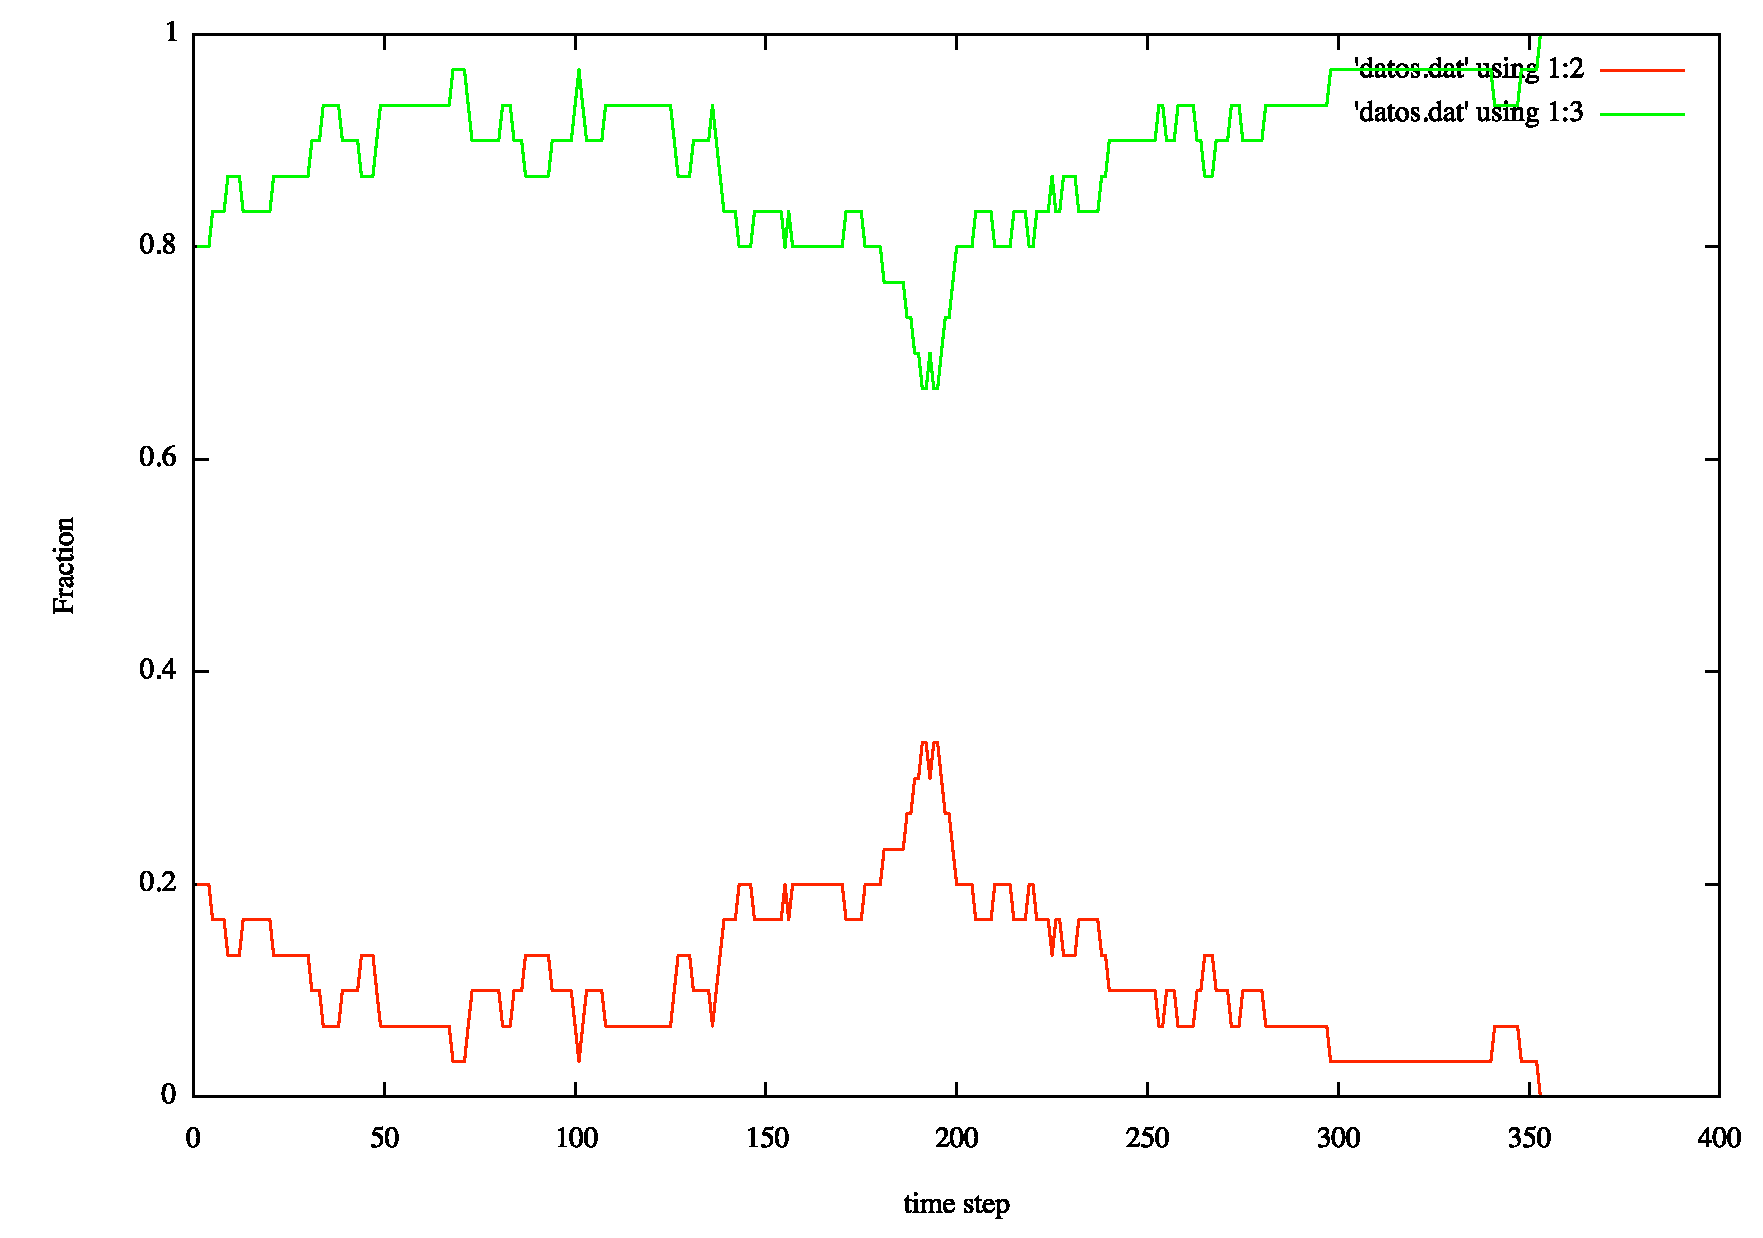
\includegraphics[width=2.5in]{bmoran1.pdf} &
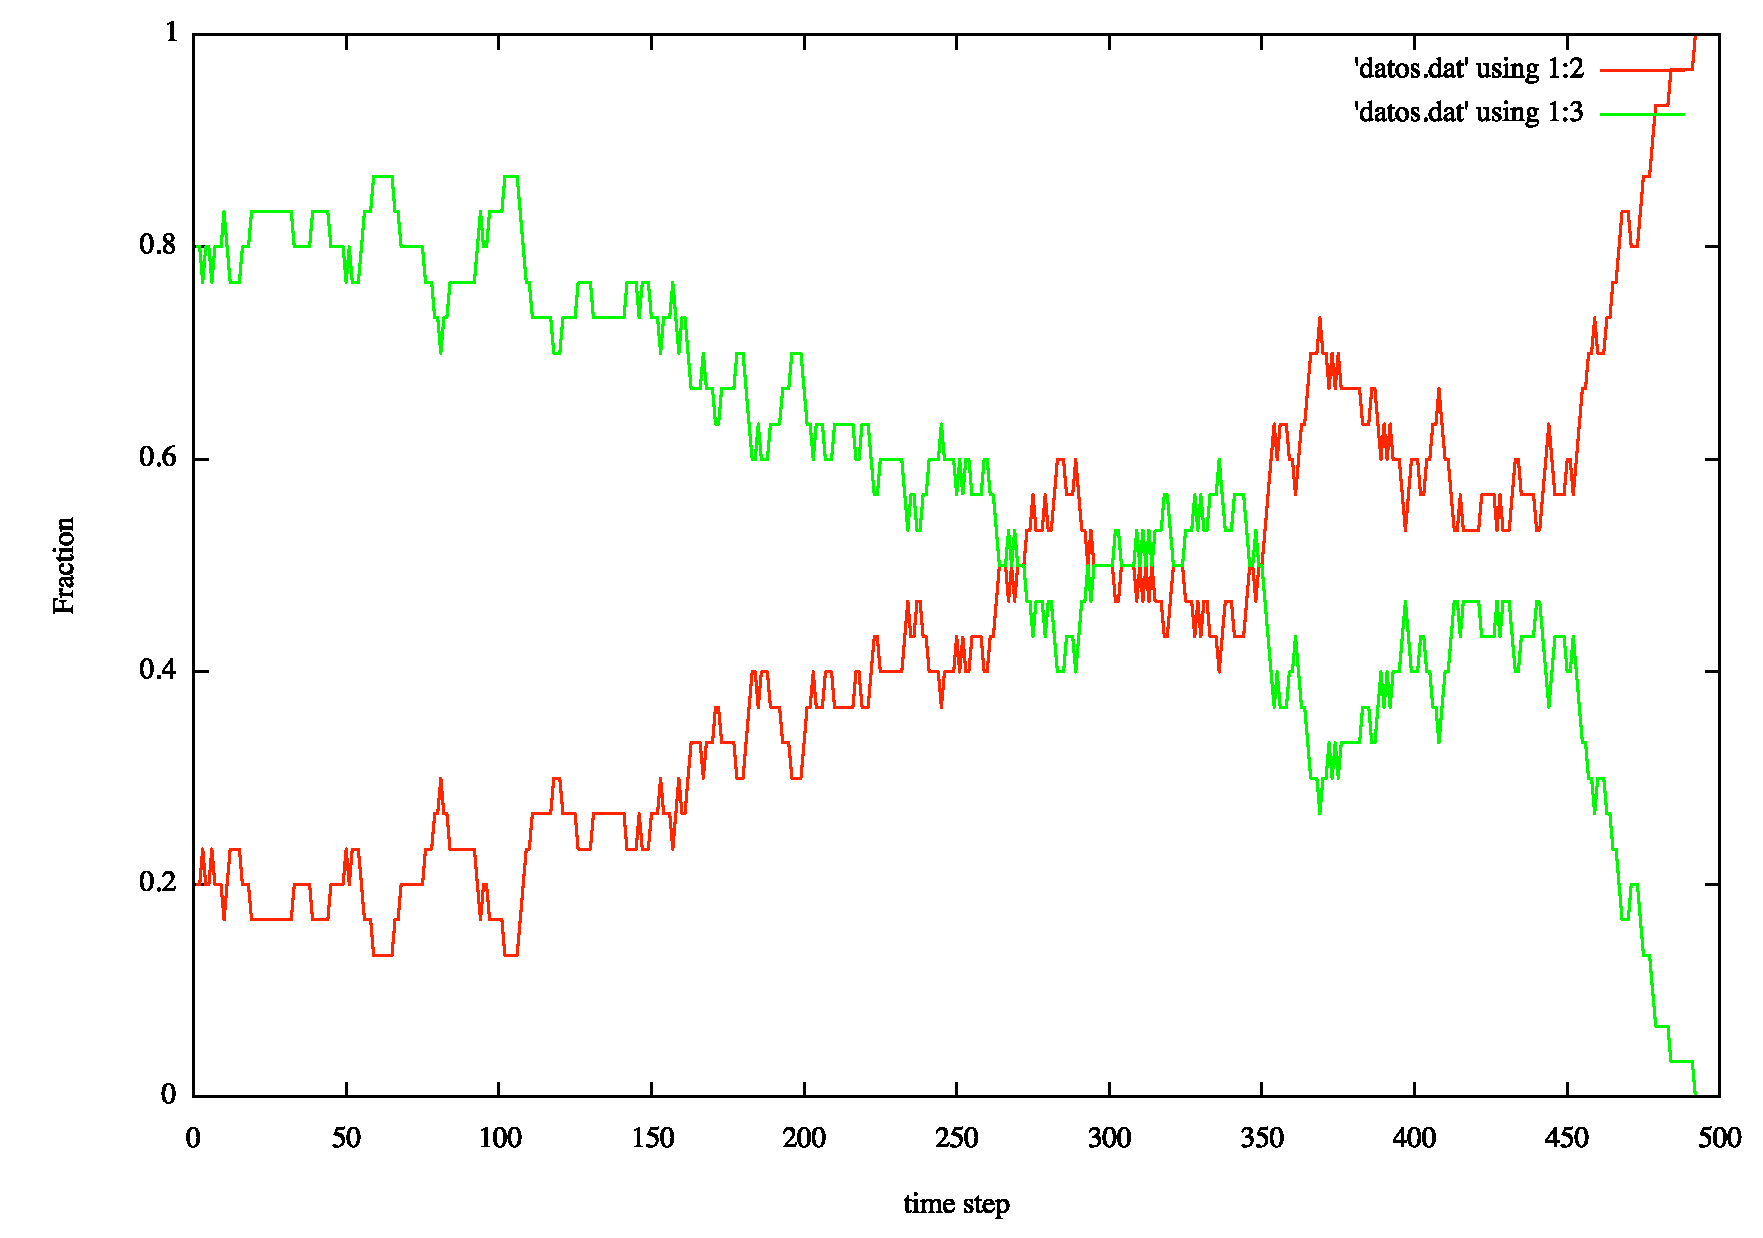
\includegraphics[width=2.5in]{bmoran.pdf}
\end{array}$
\end{center}
\caption{Two executions of the same neutral drift simulation with two different dominance result, which is due to stochasticity.}
\label{Fig46}
\end{figure}

This result for the probability $\rho_i$ can be corroborate  with the simulation shown in the next Figure (\ref{Fig47}).
\begin{figure}[H]
  \begin{center}
    \leavevmode
    \ifpdf
      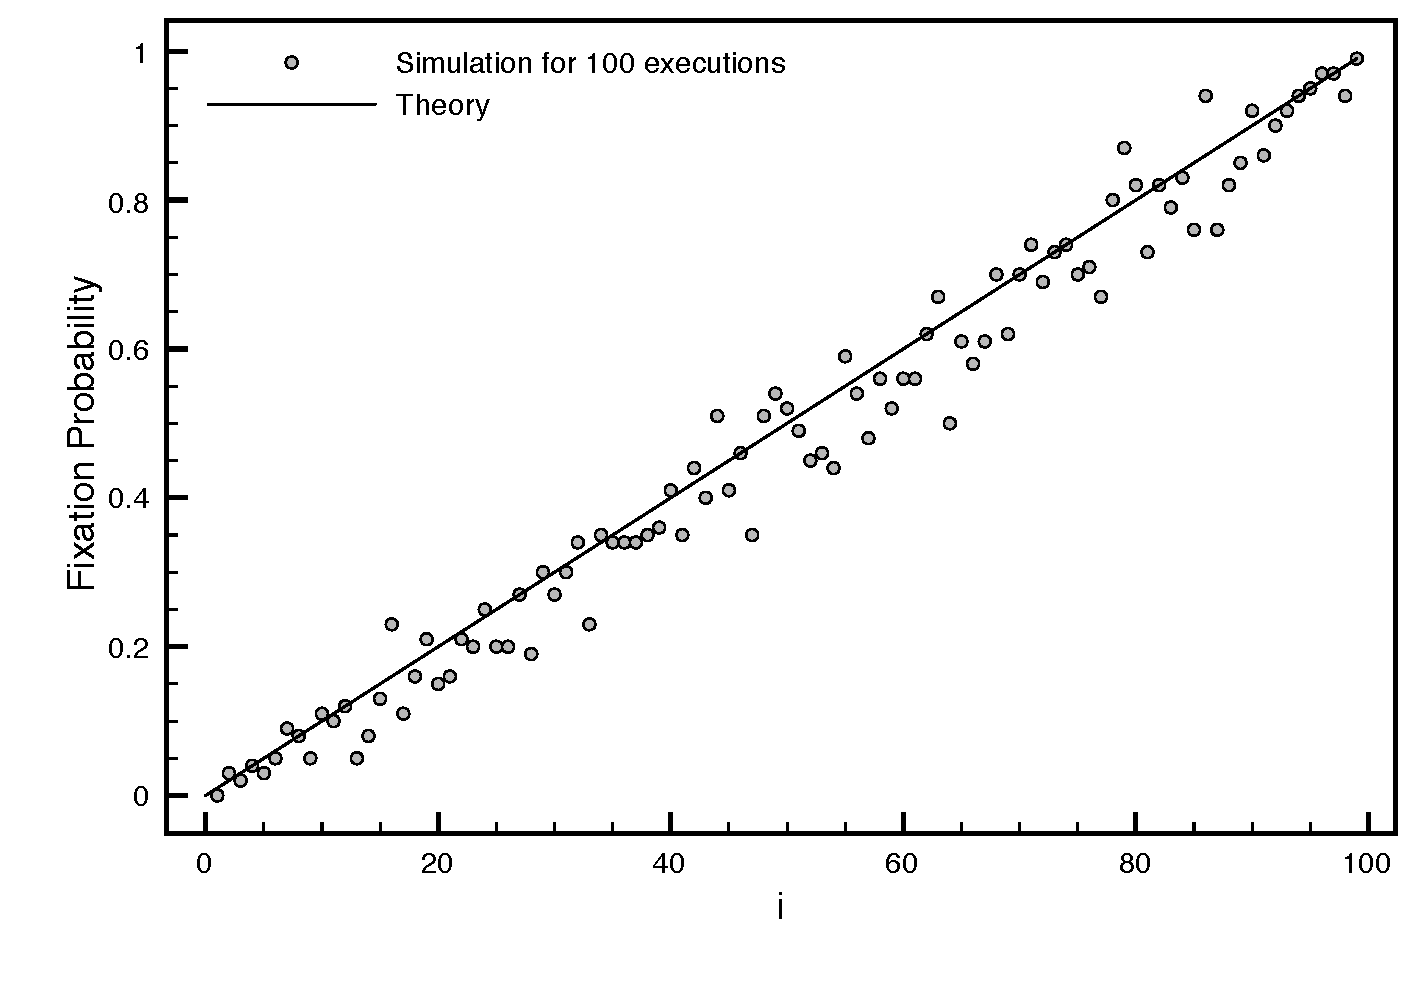
\includegraphics[width=8cm,height=7cm]{NeutralDriftPro.pdf}
    \else
      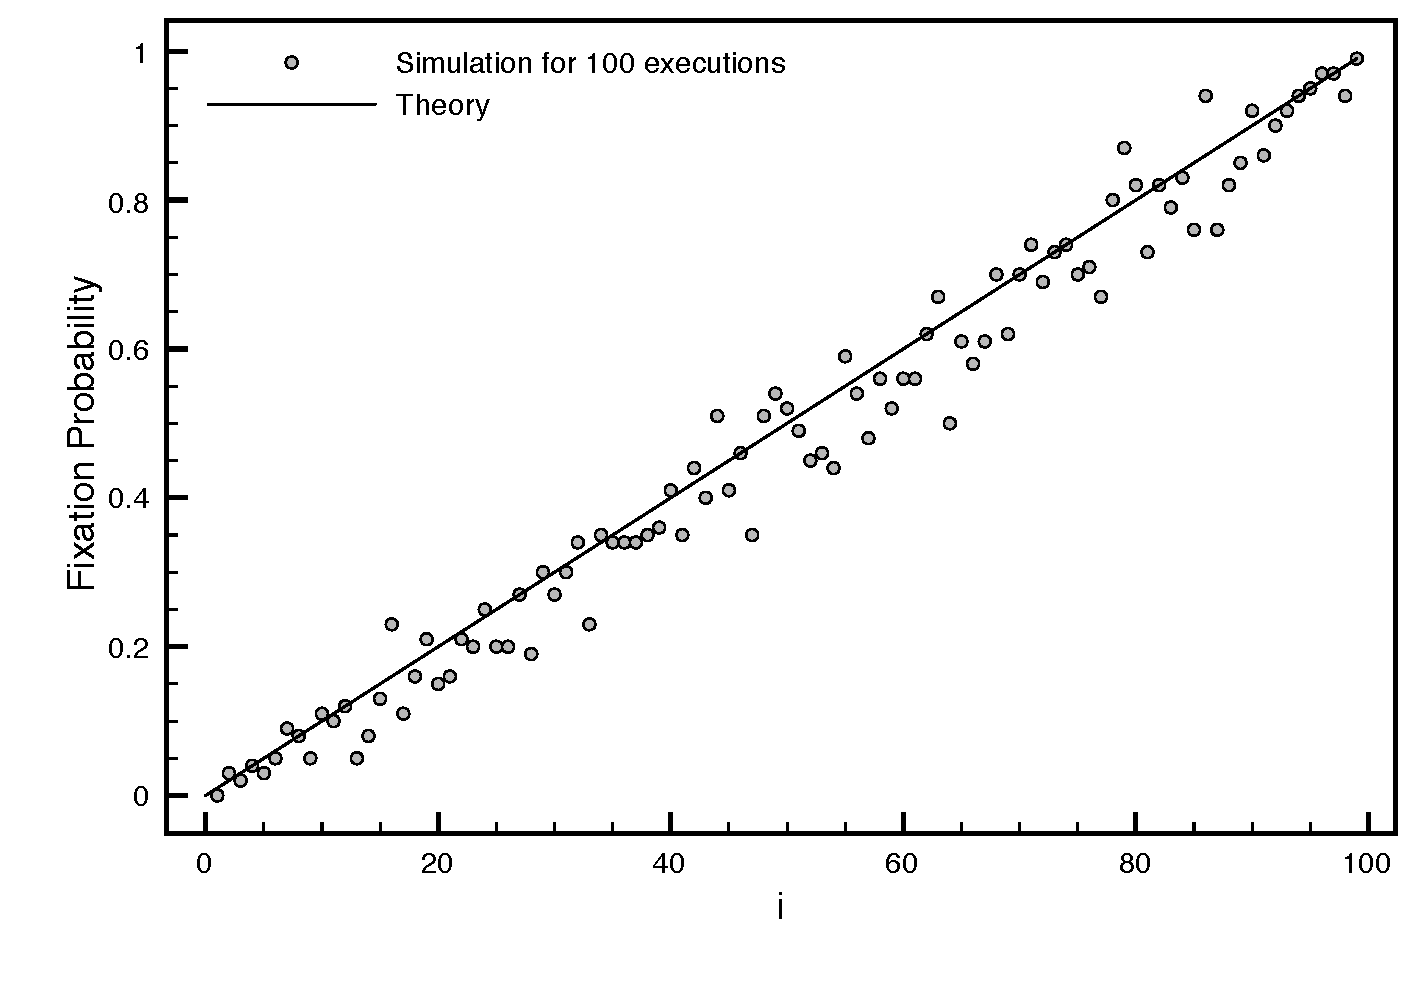
\includegraphics[width=8cm, height=7cm]{NeutralDriftPro.pdf}
    \fi
    \caption{Fixation probability in neutral drift as a function of initial population $i$ and size $n=100$.}
    \label{Fig47}
  \end{center}
  \end{figure}

\section{Random Drift}
We can perform the same calculation for the same process as before, but assuming that type $1$ has fitness $r$ and type $0$ fitness $1$. Then the probability that $1$ is chosen for reproduction is
\begin{equation}
\frac{ri}{ir+n-i}
\end{equation}
that $1$ is chosen for elimination is
\begin{equation}
\frac{i}{n}.
\end{equation}
Type $0$ has probability for reproduction $n-i/(ri+n-i)$ and $n-i/n$ for elimination. Therefore the probabilities of transition are
\begin{equation}
p_{i,i+1}=\frac{ri}{ri+n-i}\frac{n-i}{n}
\end{equation}
\begin{equation}
p_{i,i-1}=\frac{n-i}{ri+n-i}\frac{i}{n}
\end{equation}
\begin{equation}
p_{i,i}=1-p_{i,i+1}-p_{i,i-1}.
\end{equation}
Once again the conditions for fixation probabilities $\rho_{i}$ are $\rho_{0}=0$, $\rho_{n}=1$ and
\begin{equation}
\rho_{i}=p_{i,i}\rho_{i}+p_{i,i+1}\rho_{i+1}+p_{i,i-1}\rho_{i-1}.
\end{equation}
 With the new variable $y_{i}=\rho_{i}-\rho_{i-1}$ we can write equation (18) as
 \begin{equation}
 y_i = y_{i+1}\frac{p_{i,i+1}}{p_{i,i-1}}=y_{i+1}\frac{ri}{n-i}\frac{n-i}{i}
 \end{equation}
 then $y_{i+1}=\frac{1}{r}y_i$, and these lead to
\begin{equation}
y_i =\frac{1}{r^{i-1}}\rho_1
\end{equation}  
since $1=\rho_1 (1+\sum_{m=1}^{n-1}\frac{1}{r^{m}} )$ and $\rho_i=\rho_1 (1+\sum_{j=1}^{i-1}\frac{1}{r^{j}} )$, the fixation probability is
\begin{equation}
\rho_{i}=\frac{1+\sum_{j=1}^{i-1}\frac{1}{r^j}}{1+\sum_{m=1}^{n-1}\frac{1}{r^m}}.
\end{equation}
In this expression we have a telescopic series. The sum value for a telescopic series is
\begin{equation}
\sum_{i=0}^{n}\frac{1}{x^n}=\frac{1-\frac{1}{x^{n+1}}}{1-\frac{1}{x}}.
\end{equation}  
Therefore the probability of fixation for type $1$ starting in state $i$ is
\begin{equation}\label{4.25}
\rho_i = \frac{1-1/r^i}{1-1/r^n}.
\end{equation}
This result can be checked in a Moran process simulation where  the fixation probability is measured as a function of $r$. In the Figure (\ref{Fig48}) below  the analytical curve and the stochastic measures are shown.
\begin{figure}[H]
  \begin{center}
    \leavevmode
    \ifpdf
      \includegraphics[width=8cm,height=7cm]{Plot.pdf}
    \else
      \includegraphics[width=8cm, height=7cm]{Plot.pdf}
    \fi
    \caption{Fixation probability in random drift as a function of $r$ in a population of size $n=100$ and initial state $i=50$ ,where each point was calculated with $1000$ executions. The line represents the analytical model.}
    \label{Fig48}
  \end{center}
  \end{figure}
In the case where type $0$ has a fitness $s$, the fixation probability Eq. \eqref{4.25} is written as
\begin{equation}
\rho_i = \frac{1-(s/r)^i}{1-(s/r)^n}
\end{equation}
\section{Fixation Times}
Fixation time is the average time that the competition system takes to get to one of the two absorbing states\cite{Antal, Traulsen2009}. Because of the stochasticity of the system the time for reaching these states is a distribution, where each time $t$ for reaching an absorbing state($0$ or $n$) starting from $i$ type $A$ individuals has a probability $P_i ^{n,0} (t)$. As for fixation probabilities, for $P_i ^{n,0} (t)$ there is also a recurrence equation, that is the probability sum of three different events:
\begin{itemize}
\item The probability of jump to state $i-1$ in the first time step, and from there it takes a time $t-1$ with probability $P_{i-1}^{n,0}(t-1)$ for reaching the absorbing state.
\item The probability of jump to state $i+1$ in the first time step, and from there it takes a time $t-1$ with probability $P_{i+1}^{n,0}(t-1)$ for reaching the absorbing state.
\item The probability of staying in state $i$ in the first time step, and from there it takes a time $t-1$ with probability $P_{i}^{n,0}(t-1)$ for reaching the absorbing state.
\end{itemize}
 The recurrence equation is
 \begin{equation}
 P_i ^{n,0} (t)= P_{i,i-1}P_{i-1}^{n,0}(t-1)+P_{i,i+1}P_{i+1}^{n,0}(t-1)+P_{i,i}P_{i}^{n,0}(t-1).
 \end{equation}  
The probability of time $t$ for reaching state $n$ is $P_{i}^{n}(t)$, and the recurrence equation for the dominance of type $A$ is\cite{Antal}
 \begin{equation}\label{4.27}
 P_i ^{n} (t)= P_{i,i-1}P_{i-1}^{n}(t-1)+P_{i,i+1}P_{i+1}^{n}(t-1)+P_{i,i}P_{i}^{n}(t-1)
 \end{equation} 
 with the boundary conditions  $P_{0}^{n}(t)=0$ and $P_{n}^{n}(0)=1$. The average absorbsion time is
 \begin{equation}
 t_i = \frac{\sum\limits_{t=0}^{\infty}tP_{i}^{n}(t)}{\sum\limits_{t=0}^{\infty}P_{i}^{n}(t)},
 \end{equation}
 where $\sum\limits_{t=0}^{\infty}P_{i}^{n}(t)=\rho_i $.
 Multiplying Eq. \eqref{4.27} by $t$,  sum it and applying the  identity
 \begin{equation}
 \sum\limits_{t=0}^{\infty}tP_{i}^{n}(t-1)=\rho_{i}(t_i + 1).
 \end{equation}
 We get
 \begin{equation}
 t_i \rho_i =P_{i,i-1}\rho_{i-1}(t_{i-1}+1) + P_{i,i+1}\rho_{i+1}(t_{i+1}+1) + P_{i,i}\rho_{i}(t_{i}+1).
 \end{equation}
 Replacing $\tau_{i}=t_i \rho_i$ and using the recurrence equation Eq. \eqref{4.9}, the above equation becomes
 \begin{equation}
 -\rho_i =P_{i,i-1}\tau_{i-1}-\tau_1(P_{i,i+1}+P_{i,i-1})+P_{i,i}\tau_{i+1}.
 \end{equation}
 Because this is a recurrence relation we can use $s_{i}=\tau_i -\tau_{i+1}$, and get
 \begin{equation}
 s_{i}=\frac{P_{i,i-1}}{P_{i,i+1}}s_{i-1}+\frac{\rho_i}{P_{i,i+1}}.
 \end{equation}
 since $s_{0}=-\tau_1$, and iterating some times:
 \begin{equation*}
 \begin{split}
s_1 = & \frac{\rho_1}{P_{1,2}} - t_1 \rho_1\frac{P_{1,0}}{P_{1,2}} \\
:\\
s_3 =& \frac{P_{3,2}}{P_{3,4}}\left[\frac{P_{2,1}}{P_{2,3}}\left( \frac{\rho_{1}}{P_{1,2}}+  s_0 \frac{P_{1,0}}{P_{1,2}}\right)+ \frac{\rho_2}{P_{2,3}}\right] + \frac{\rho_{3}}{P_{3,4}}.
 \end{split}
\end{equation*}
Then by induction:
\begin{equation}\label{4.33}
s_{i}=s_0 \prod\limits_{j=1}^{i}\frac{P_{j,j-1}}{P_{j,j+1}} + \sum\limits_{j=1}^{i}\frac{\rho_j}{P_{j,j+1}}\prod\limits_{m=j+1}^{i}\frac{P_{m,m-1}}{P_{m,m+1}},
\end{equation}
with the convention that $\prod\limits_{i+1}^{i}\frac{P_{m,m-1}}{P_{m,m+1}} =1$.
Now to determinate $t_1$, we use the fact that $\sum\limits_{n=1}^{i}s_n = \tau_1-\tau_{i+1}$, and $\tau_n=0$.Then 
\begin{equation}
\tau_1=\sum\limits_{i=1}^{n-1}s_i,
\end{equation}
and using Eq. \eqref{4.33}
\begin{equation}
\tau_1\left(1+ \sum\limits_{i=1}^{n-1}\prod\limits_{j=1}^{i}\frac{P_{j,j-1}}{P_{j,j+1}}\right)=\sum\limits_{i=1}^{n-1}\sum\limits_{j=1}^{i}\frac{\rho_j}{P_{j,j+1}}\prod\limits_{m=j+1}^{i}\frac{P_{m,m-1}}{P_{m,m+1}},
\end{equation}
Finally $t_{1}$ is
\begin{equation}\label{4.36}
t_1=\sum\limits_{i=1}^{n-1}\sum\limits_{j=1}^{i}\frac{\rho_j}{P_{j,j+1}}\prod\limits_{m=j+1}^{i}\frac{P_{m,m-1}}{P_{m,m+1}}.
\end{equation}
With this result we can determinate the expression for the fixation time $t_{i}$ of $i$ initial $A$ individuals. We can see that 
\begin{equation}
\sum\limits_{k=1}^{i-1}s_k=\tau_1 -\tau_i,
\end{equation}   
but in this equation we can replace
\begin{equation*}
\sum\limits_{k=1}^{i-1}s_k=\sum\limits_{k=1}^{n-1}s_k -\sum\limits_{k=i}^{n-1}s_k
\end{equation*} 
to get the relation
\begin{equation}
\tau_i=\sum\limits_{k=i}^{n-1}s_k
\end{equation}
where replacing $s_k$.  $t_i$ is
\begin{equation}\label{4.39}
t_i=-\frac{\rho_1 t_1}{\rho_i}\sum\limits_{k=i}^{n-1}\prod\limits_{j=1}^{k}\frac{P_{j,j-1}}{P_{j,j+1}} + \sum\limits_{k=i}^{n-1}\sum\limits_{j=1}^{k}\frac{\rho_j}{\rho_i P_{j,j+1}}\prod\limits_{m=j+1}^{k}\frac{P_{m,m-1}}{P_{m,m+1}}.
\end{equation}
For random drift $t_1$ and $t_i$ simplify to:
\begin{equation}
t_{1}=\frac{n}{1-(\frac{s}{r})^n}\sum\limits_{k=1}^{n-1}(\frac{s}{r})^k \sum\limits_{l=1}^{k}\left(1-(\frac{s}{r})^l \right)\left(\frac{1}{n-1}+\frac{s}{rl}\right),
\end{equation}
\begin{equation}
t_i=t_1 -t_1\left(\frac{1-(s/r)^n}{1-(s/r)^i}\right)+\frac{n}{r(1-(s/r)^i)}\sum\limits_{k=i}^{n-1}\sum\limits_{l=1}^{k}\left(1-(s/r)^l\right)\frac{(rl+s(n-l))}{l(n-l)}
\end{equation}
If we observe carefully these expressions, it can be seen that $t_1$ is shorter as fitness $r$ increases. In the case for $t_{i}$, the larger the initial population $i$, the shorter the average time for reaching dominance. These interpretations are consistent  with those from Eq. \eqref{3.12}. 
% ------------------------------------------------------------------------


%%% Local Variables: 
%%% mode: latex
%%% TeX-master: "../thesis"
%%% End: 
